
This section will introduce and develop the \rrtfunnel{} algorithm, by two
means: First develop robust motion primitives through the \ac{SOS} programming
framework based on the work by \cite{majumdarFunnelLibrariesRealtime2017}, and
second, deploy these funnels as robust motion primitives in a discrete \ac{RRT}
robust motion planner based on \cite{Lav06}. Using robust motion primitives has
several advantages. Firstly, they handle uncertainty, and thus, as long as the
uncertainties in the system are akin to the assumptions on the incoming
uncertainty parameters, the dynamical system will not leave the funnel, and
hence if the funnel is not in collision, neither will the system be. Secondly,
as the motion primitives are robust, there is no need for more conservative
maneuvers and heuristics, such as maximizing the distance to an obstacle, which
is a naive way for motion planners to handle uncertainty. Since the primitives
are robust, the system might as well choose a primitive that is close to an
obstacle, as one that is far away, since the funnel is guaranteed to be
collision-free in both cases. This means that a robust motion algorithm can
perform more aggressive maneuvers than one that is inherently conservative about
its environment and maneuvers~\cite{singhRobustOnlineMotion2017}.


\subsection{Generating Robust Motion Primitives}
\label{sec:generating-robust-motion-primitives}

This paper employs the simple unicycle model from
\author{Lav06}~\cite[613]{Lav06} which is modified slightly into
\begin{equation}
  \label{eq:model-dynamics}
  \vect{x} =
  \begin{bmatrix}
    x \\ y \\ \theta \\
  \end{bmatrix}, \, \dot{\vect{x}} =
  \begin{bmatrix}
    -v \sin(\theta) \\
    v \cos(\theta) \\
    u \\
  \end{bmatrix}
  ,
\end{equation}
which is a first-order unicycle model with a constant speed of \(v=10\)
\IEEEunit{m/s}. Although this is the only model used in this paper, the
framework and the code is easily adapted into accommodating a different and more
complicated model.


\subsubsection{Generating Trajectories}
\label{subsec:generating-the-trajectories}

The robust motion primitives are \textit{finite regions of time variance} around
an initial trajectory, meaning that they are all the states surrounding a
trajectory in which the system can reach in a given time. But in order to verify
the robust regions surrounding a trajectory, first the trajectories themselves
have to be generated. Generating optimal trajectories is a rich field in the
motion planning literature~\cite{Betts_1998}. The initial trajectories can be
generated by many different methods, however the \textit{direct collocation
method} suited the needs of this paper best~\cite{von1993numerical}. It was
chosen as it builds locally optimal trajectories from a discrete set of sampled
points along a sought trajectory, which is beneficial for the discrete funnel
verification in \cref{subsec:generating-funnels}. For this problem the cost
function chosen for the solver to minimize is:
\begin{equation}
  J = \int_{0}^{T} \left[ 1 + {\vect{u}_{0}}^{T} \matr{R} \vect{u}_{0} \right] \mathrm{d}t,
\end{equation}
where \(\matr{R} = 1\), because it will minimize the system input, and thus give
a smooth output trajectory~\cite{majumdarRobustOnlineMotion2013}.

\subsubsection{Initializing the Funnel Calculations}
\label{subsec:initializing-tvlqr}

The funnel calculation algorithm has to be initialized with a candidate Lyapunov
function. In the same way as in
\citeauthor{majumdarRobustOnlineMotion2013}~\cite{majumdarRobustOnlineMotion2013},
the funnel generation algorithm will be initialized with a \ac{TV-LQR}
controller as the initial Lyapunov function employing a cost function of the
form
\begin{IEEEeqnarray*}{ll}
  J &= \vect{x}^{T} (t_f) \matr{F}(t_f) \vect{x} (t_f) \IEEEyesnumber \\
    &+ \int_{t_{0}}^{t_{f}} \left( \vect{x}^{T} \matr{Q} \vect{x} + \vect{u}^{T} \matr{R} \vect{u} + 2 \vect{x}^T \matr{N} \vect{u} \right) \mathrm{d}t,
\end{IEEEeqnarray*}
which when employed on the linearization of the system error
dynamics in Equation~\eqref{eq:system-error-dynamics} gives
\begin{equation}
  \dot{\bar{\vect{x}}} \approx \matr{A} (t)\bar{\vect{x}}(t) + \matr{B}(t) \bar{\vect{u}}(t)
\end{equation}
\begin{equation}
  \dot{\bar{\vect{x}}} \approx %
  \begin{bmatrix}
    0 & 0 & -v\cos(\theta) \\
    0 & 0 & -v\sin(\theta) \\
    0 & 0 & 0 \\
  \end{bmatrix} %
  \bar{\vect{x}} (t) %
  + %
  \begin{bmatrix}
    0 \\ 0 \\ 1
  \end{bmatrix} %
  \bar{\vect{u}}(t),
\end{equation} 
which is an an initial candidate Lyapunov function of the form
\begin{equation}
  V(t,\bar{\vect{x}}) = {\bar{\vect{x}}}^{T} \matr{S}_{i}\bar{\vect{x}} ,
\end{equation}
where \(S_{i}\) is a solution of the \textit{Ricatti} equation
\begin{IEEEeqnarray*}{Cr}
  \label{eq:ricatti}
  - \dot{\matr{S}}(t) = \matr{A}^{T} \matr{S}(t) +\matr{S}(t) \matr{A} - \left( \matr{S}(t) \matr{B} + \matr{N} \right) \matr{R}^{-1} \IEEEyesnumber \\
  \IEEEeqnarraymulticol{2}{r}{\left( \matr{B}^{T} \matr{S}(t) + \matr{N}^{T} \right) + \matr{Q}}
\end{IEEEeqnarray*} 
associated with the \ac{LQR} controller. The feedback is gained from
\[
  \matr{K}(t) = \matr{R}^{-1} \left( \matr{B} \matr{S}(t) + \matr{N}^T \right),
\]
and enables the system dynamics \cref{eq:model-dynamics} to be written
\(f_{\mathit{cl}}(t,\vect{x})\) by direct substitution of \(\vect{u} =
-K\vect{x}\), where \(K\) is a \(1 \times 3\) matrix, and hence making the system in \cref{eq:model-dynamics} 
dependent only on \(t\) and \(\vect{x}\),
\begin{equation}
  \label{eq:model-dynamics-cl}
  \vect{x} =
  \begin{bmatrix}
    x \\ y \\ \theta \\
  \end{bmatrix}, \, \dot{\vect{x}} =
  \begin{bmatrix}
    -v \sin(\theta) \\
    v \cos(\theta) \\
    -K\vect{x} \\
  \end{bmatrix} \mathEoS
\end{equation}


\subsection{Generating Funnels Around Trajectories}
\label{subsec:generating-funnels}

With the nominal trajectories, and the initial Lyapunov functions ready, the
funnels around the nominal trajectories can be calculated using
\cref{alg:funnelalgorithm} on page~\pageref{alg:funnelalgorithm}, and is
implemented in software through the \textsc{sostools}~\cite{sostools} toolbox.

However, the dynamics for the model in \cref{eq:model-dynamics-cl} are still not
polynomial, given the \(\sin\) and \(\cos\) terms
in~\eqref{eq:model-dynamics-cl}, and the \ac{SOS}-framework can only verify
polynomial systems. Thus in order to obtain the needed polynomial dynamics, the
system is expanded around the nominal trajectory with a Taylor expansion of
degree three. The function limiting the size of the funnel \(\rho(t_{k})\) also
has to be initialized by a feasible upper bound \(\rho(t)\). This is done
through the equation
\begin{equation}
  \rho(t_{k}) = \mathrm{exp}\left( \rho_{\tau}\frac{\left( t_{f} - t \right)}{\left( t_{f} - t_{0}  \right)}\right) + \rho_0
\end{equation}
where \(\rho_{\tau}\) is a positive constant determining the upper bound on the
funnel, along with the zero value \(\rho_0\). If the given choice of
\(\rho_{\tau}\) does not verify a funnel, either increase the value of
\(\rho_{\tau}\) and \(\rho_0\), and optionally the number of sampled points from
the trajectory to be verified~\cite{Tobenkin_2011}.

The initial condition set also has to be decided before the reachable set can be
calculated. In general the initial condition set can be any semi-algebraic set
in the state-space. However, a simple way of obtaining an initial condition set
for the trajectories at hand is by taking advantage of the Lyapunov function
candidate from the \ac{LQR}-controller~\cite{tedrakeLQRtreesFeedbackMotion2009}.
Thus by setting
\begin{equation}
  \mathcal{X}_{0} = \frac{ \matr{S}_{k}}{\rho_{\tau}},
\end{equation}
an initial condition set is obtained. In general however, any semi-algebraic set
will do, and the algorithm is not constrained to this one initial condition set
in particular, but it has proven itself useful when calculating new motion
primitives for a system when the initial condition set is not obvious. Another
idea is to use the outlet of one funnel as the initial condition set for the
calculation of the next.

The funnels in this paper are parameterized as sub-level sets of a Lyapunov
function for which the state-space does not invalidate the sub-level constraint.

However, for the funnels in this paper, the initial condition set will be given
by the hyper-ellipsoid
\begin{align}
  \mathcal{X}_0 &= \set{\vect{x} \in \R^{3} \mid \vect{x}^{T} Q \vect{x}} \\
  Q &= \begin{bmatrix}
    2 & 0 & 0 \\
    0 & 2 & 0 \\
    0 & 0 & 4
  \end{bmatrix} \mathEoS
\end{align}


\subsection{Optimization of the Nominal \ac{LQR}-Controller}
\label{subsec:searching-for-a-controller}

With the non-optimal feedback controller given to the funnel calculation
framework (non-optimal with regards to the funnel calculation cost function),
the size of the funnels will in general be larger than if the optimizer is given
a better controller. Thus in order to further minimize the size of the funnel in
the xy-plane, this method, along with the cost function from
\cref{subsec:xy-cost-function} is used to make traversal through obstacles in
the world space easier, through minimizing the size of the reachable set. Hence,
the initial controller fed to the algorithm can be optimized with the goal of
minimizing the size of the funnel, given a few conditions on the
system.

In order for the controller to be optimized, the system needs to be control
affine, i.e. it can be written on the form
\begin{equation}
  \dot{\vect{x}} = f(\vect{x}(t)) + g(\vect{x}(t)) \vect{u} (t),
\end{equation}
so that the control policy can be parameterized as a polynomial
\(\bar{\vect{u}}_f(t,\bar{\vect{x}})\), and the system dynamics written as
\begin{equation}
  \dot{\bar{\vect{x}}} = f(\vect{x}_0(t) + \bar{\vect{x}}(t)) + g(\vect{x}(t))\left( \vect{u}_0(t) + \bar{\vect{u}}_f(t,\bar{\vect{x}}) \right) - \bar{\vect{x}}_0 \mathEoS \label{eq:dynamics-control-affine}
\end{equation}
Given that the dynamical model in \cref{eq:model-dynamics} is control affine,
since
\begin{IEEEeqnarray*}{rl}
  \dot{\vect{x}} &= %
  f(\vect{x}(t)) + g(\vect{x}(t)) \vect{u} (t) \IEEEyesnumber \\
  &= %
  \begin{bmatrix}
    -v(t)\sin (\theta) \\
    v(t) \cos (\theta) \\
    0
  \end{bmatrix}
  +
  \begin{bmatrix}
    0 \\
    0 \\
    1 \\
  \end{bmatrix}
  \vect{u}(t),
\end{IEEEeqnarray*}
the feedback controller can be optimized by adding the coefficients of the
polynomial \(\vect{u}_f(t,\bar{\vect{x}})\) to the set of decision variables in
the original optimization
problem~\eqref{opt:discrete}~\cite[sec~4.3.2]{majumdarFunnelLibrariesRealtime2017}.
The only issue is that now \(\dot{V}\) is bilinear in the decision variables
\(V\) and \(\bar{\vect{u}}_f\), as well as the other bilinear decision variables
from the \cref{opt:time-dependent-optimization-problem}, as can be seen from
\begin{equation}
  {
    \dot{V}(t,\vect{x}) = \frac{\partial V(t,\vect{x})}{\partial \vect{x}} \dot{\bar{\vect{x}}} + \frac{\partial V(t,\vect{x})}{\partial t},
  }
\end{equation}
where \(\dot{\bar{\vect{x}}}\) is now given by
\cref{eq:dynamics-control-affine}. Thus in order to optimize the control input a
search is done in the variables \( (\bar{\vect{u}}_f,\rho,L_t,L_{0,i},S_k) \)
while keeping \( (V,L,L_{\epsilon,k}) \) fixed. This method combined with the
uncertainty added in~\cref{sec:adding-uncertainty}, is what forms the basis for
the funnel computations as robust motion primitives for traversal in a dense
forest environment, as summarized in \cref{alg:funnelalgorithm-extended}
(Optimization 2).

A figure of a straight funnel motion primitive calculated with uncertainties by
the \ac{SOS} solver can be seen in \cref{fig:funnel-calculation-visuals}.

\begin{figure}[!t]
  \centering 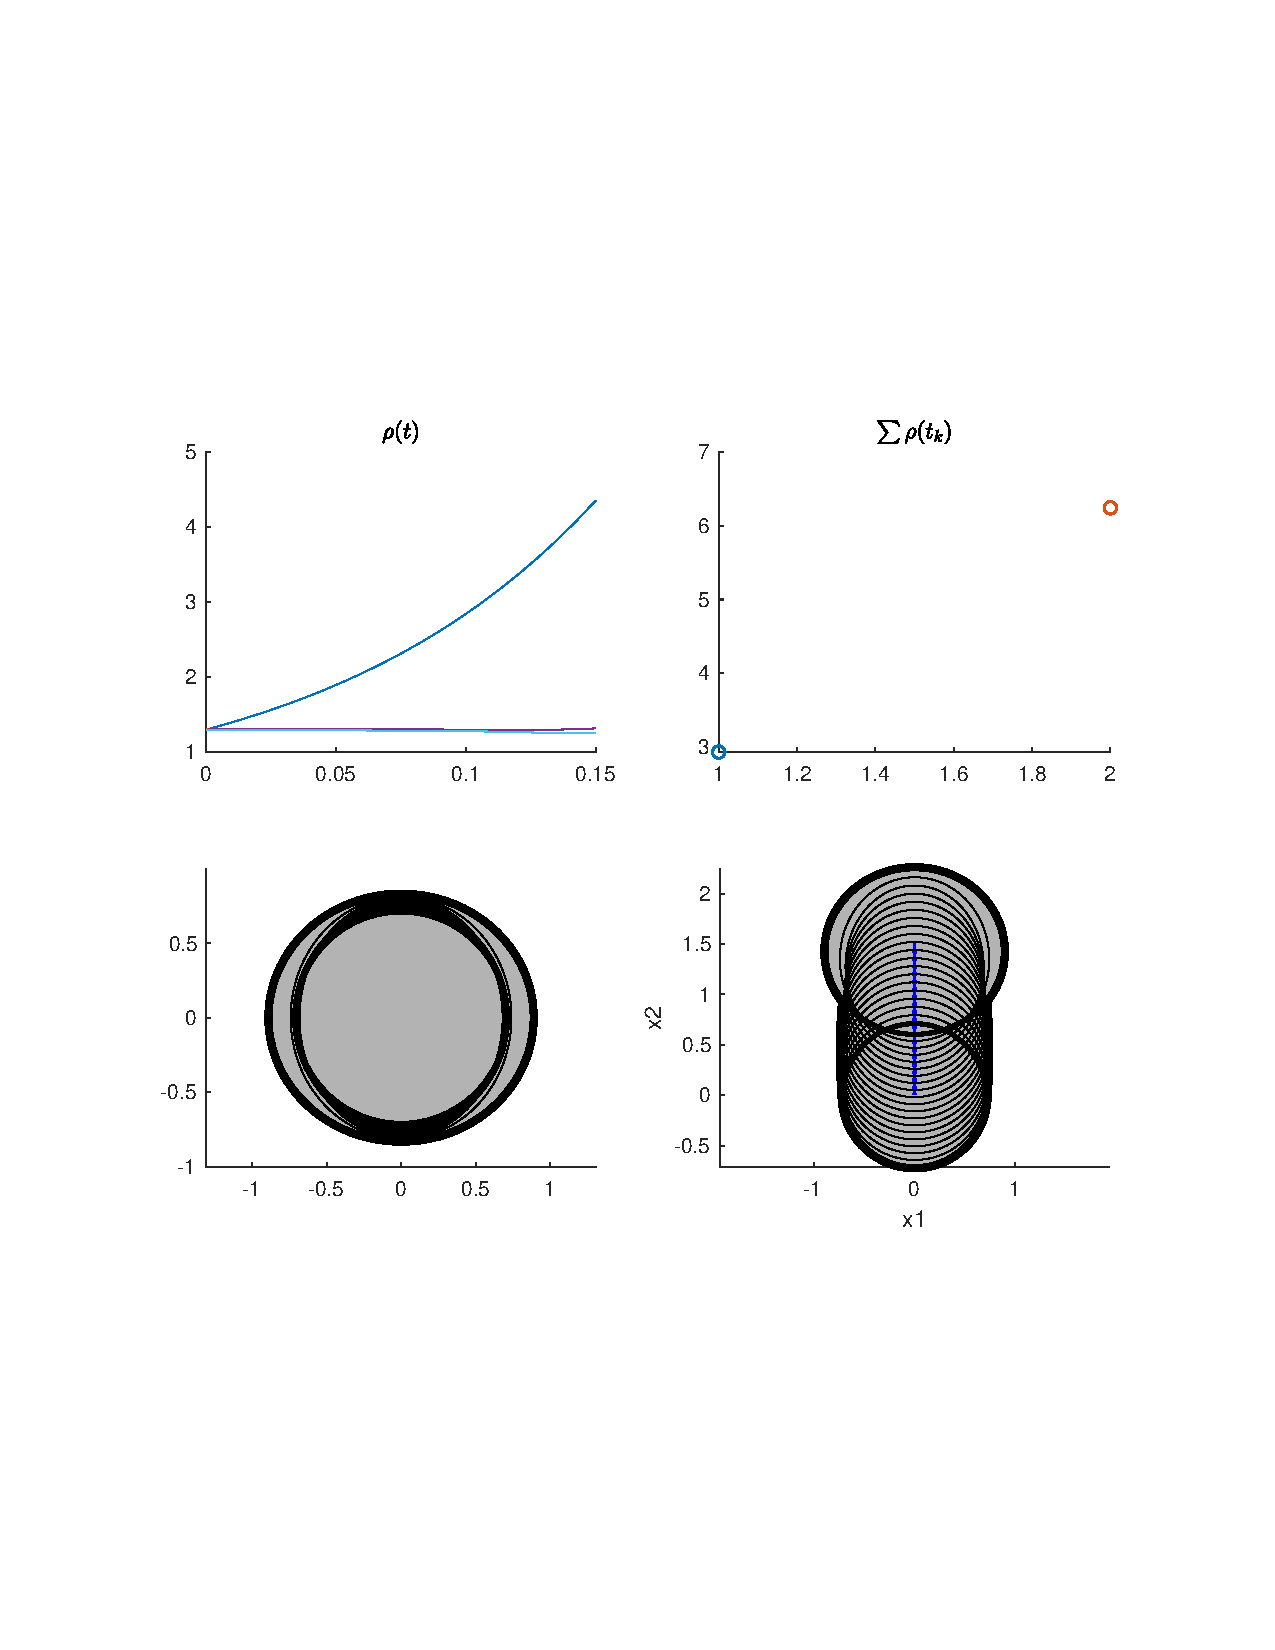
\includegraphics[width=\linewidth, scale=.5, trim={0cm 6cm 0cm
    6cm}]{figures/method/funnel-calculation-visuals}
  \caption[A funnel calculated around a straight trajector]{A funnel calculated
    around a straight motion trajector. Shown is the value of \(\rho(t)\), and
    \(\sum \rho(t_k)\) as it is incrementally improved by the numerical solver.
    The bottom figures are the funnel projected down in the xy-plane. The left
    the ellipsoids are overlaid on top of each other, and on the right they are
    plotted on top of their respective sampling points in time \(t_k\).}
  \label{fig:funnel-calculation-visuals}
\end{figure}


\subsection{Funnel Transformations and Invariance}
\label{subsec:shifting-funnels}

Now that the funnels are able to be calculated for a basic set of motion
primitives, it is time to start looking at chaining these primitives together in
order to construct longer and more complex motions from a basis of motion
primitives. Thus, in order to freely shift funnels around in the configuration
space, the cyclic coordinates of the system have to be determined, so that the
dynamics of the system is never violated. Even though the funnels can now start
and end in a completely different part of the configuration space, the original
dynamics must not be violated. Therefore the cyclic and non-cyclic coordinates
of the system must be decided. This is done through finding the cyclic and
non-cyclic coordinates through the method from \cref{subsec:cyclic-coordinates}.
Therefore, given the model from \cref{eq:model-dynamics} the cyclic coordinates
of the system are found from:
\begin{align*}
  \mathcal{L} &= T - V = \frac{1}{2} mv^2 + \frac{1}{2}I\dot{\theta}^2 \\ 
              &= \frac{1}{2} \left(  m \left(
                \dot{\vect{x}}^2 \sin^2 \theta + \dot{\vect{x}}^2 \cos^2 \theta
                \right)  + I {\dot{\theta}}^2 \right) \\
              &= \frac{1}{2} \left(  m\dot{\vect{x}}^2 + I {\dot{\theta}}^2 \right)
\end{align*}
which shows that the Lagrangian is invariant to shifts in the \((x,y,\theta)\)
variables, since \(\frac{\partial\mathcal{L}}{\partial q_i} = 0, \, q_i =
x,y,\theta\). Now any funnel in the base set can be shifted freely around in the
cyclic coordinates of the system without changing the solution to the system
dynamic equation, and thus create an infinite set of funnels in the state space
for the planner to work with. Through the partitioning of coordinates into
cyclic- and non-cyclic coordinates of the form \(\vect{x} = \left[ x_c\; x_{nc}
\right]^{T }\), the state dynamics \cref{eq:model-dynamics} only depends on the
cyclic coordinates of the system. Thus, a trajectory of the form \(t \rightarrow
\bigl( \vect{x}(t), \vect{u}(t) \bigr) \) which solves \(\dot{\vect{x}} = f
\bigl(\vect{x}(t), \vect{u}(t) \bigl) \) can then be transformed through a shift
\(\Psi_{c}\) along the cyclic coordinates of the system to yield a valid
solution of the form
\[
  t \rightarrow \bigl( \Psi_{x}(\vect{x}(t)), \vect{u}(t) \bigr)
\]
where the transform \(\Psi\) is given by
\[
  \Psi \bigl( \begin{bmatrix}
    \vect{x}_{c}  \\ \vect{x}_{\mathit{nc}} 
  \end{bmatrix}
  \bigr) =
  \begin{cases}
    \vect{x}_{c} \rightarrow \vect{x}^{'}_{c} \\
    \vect{x}_{\mathit{nc}} \rightarrow \vect{x}_{\mathit{nc}} \mathEoS
  \end{cases}
\]
However, since \( \dim (\vect{x}) = \dim(\vect{x}_{c}) \), for
the~\cref{eq:model-dynamics}, it is not necessary to handle the non-cyclic case.


\subsection{Sequential Funnel Composition}
\label{sec:composable-funnels}

Now that funnels can be shifted freely around the configuration space along the
cyclic coordinates of the system to create new motion primitives, it is time to
start chaining funnels together to create trees of funnels that span out into
the planning environment in order to create a robust motion plan.

However, in order for two funnels to create a third and new motion primitive
when chained together, they need to be composable. This means that the inlet of
the second funnel needs to be fully contained within the outlet of the first
one. Otherwise the robustness guarantees of the traversal will be lost. An
abstract pictorial representation of two funnels composed together can be seen
in~\cref{fig:two-funnels-composed} to emphasize this observation.

The mathematical definition of funnel composition
(\cref{def:funnel-composition}) that is used to verify that two funnels are
composable is not in accordance with the new transformed funnels from
\cref{subsec:shifting-funnels}. However, take note that the definition only has
to be modified slightly in order to take into account the translation along the
cyclic coordinates of the system.
\begin{definition}
  \label{def:invarant-funnel-composition}
  An ordered pair \((F_1,F_2)\) of funnels \(F_1 \colon [0,T_1] \rightarrow
  \mathcal{P}(\R^n)\) and \(F_2 \colon [0,T_2] \rightarrow \mathcal{P}(\R^n)\)
  is \textit{sequentially composable modulo invariance} if there exists a shift
  along cyclic coordinates such that \(F_{1}(T_1) \subset
  \Psi_{c}\bigl(F_2(0)\bigr) \).
\end{definition}
In layman's terms this means that if a funnel \(F_2\) can be shifted along
cyclic coordinates to stack up against the outlet of funnel \(F_2\) so that they
are composable in the sense of \cref{def:funnel-composition}, they are
composable modulo
invariance~\cite[definition~3,sec~5]{majumdarFunnelLibrariesRealtime2017}. Since
any funnel in the configuration space will be a set consisting of the funnel
from the basic set, along with a transformation along the cyclic coordinates of
the system, the set of all funnels, \(\hat{\mathcal{F}}\), in the configuration
space, is written \(\hat{\mathcal{F}} = \set{F_n \in \R^n \mid \Psi_{c,i}(F_i),
  F_i \in \mathcal{F}}\). Here \(\mathcal{F}\) is the basic set of funnels, and
since the transformation is already known the composability is straightforward
to compute.

\begin{figure}[!t]
  \centering {
\includegraphics[width=.8\columnwidth]{figures/method/funnel-composition}}
  \caption[Two composable funnels]{Two funnels that can be successfully composed, as the outlet of the
    first one is fully contained in the inlet of the second.}
  \label{fig:two-funnels-composed}
\end{figure}

Therefore apply the generalized S-procedure on
\begin{equation}
  V_1(T_1,\bar{\vect{x}}) \leq \rho_1(T_1) \implies V_2(0, \bar{\vect{x}}) \leq \rho_2(0) \mathEoS
\end{equation}
Then the composability of two funnels can be checked through the \ac{SOS}
program
\begin{IEEEeqnarray*}{ll}
   \text{Find } L(\vect{x}) \IEEEyesnumber \\
  \text{s.t.} \\
   \IEEEeqnarraymulticol{2}{r}{\rho_2(0) - V_2(0,\vect{x}) - L(\vect{x})\left( \rho_1(T_1) - V_1(T_1,\vect{x}) \right) \text{ is SOS}} \\
  \IEEEeqnarraymulticol{2}{r}{L(\vect{x}) \text{ is SOS}} \mathEoS
\end{IEEEeqnarray*}
Which is implemented using \textsc{sostools}~\cite{sostools} and \matlab{}. For a picture of funnels composed
together into a tree have a look at \cref{fig:funnel-composition-tree}.
\begin{figure}[!t]
  \centering
  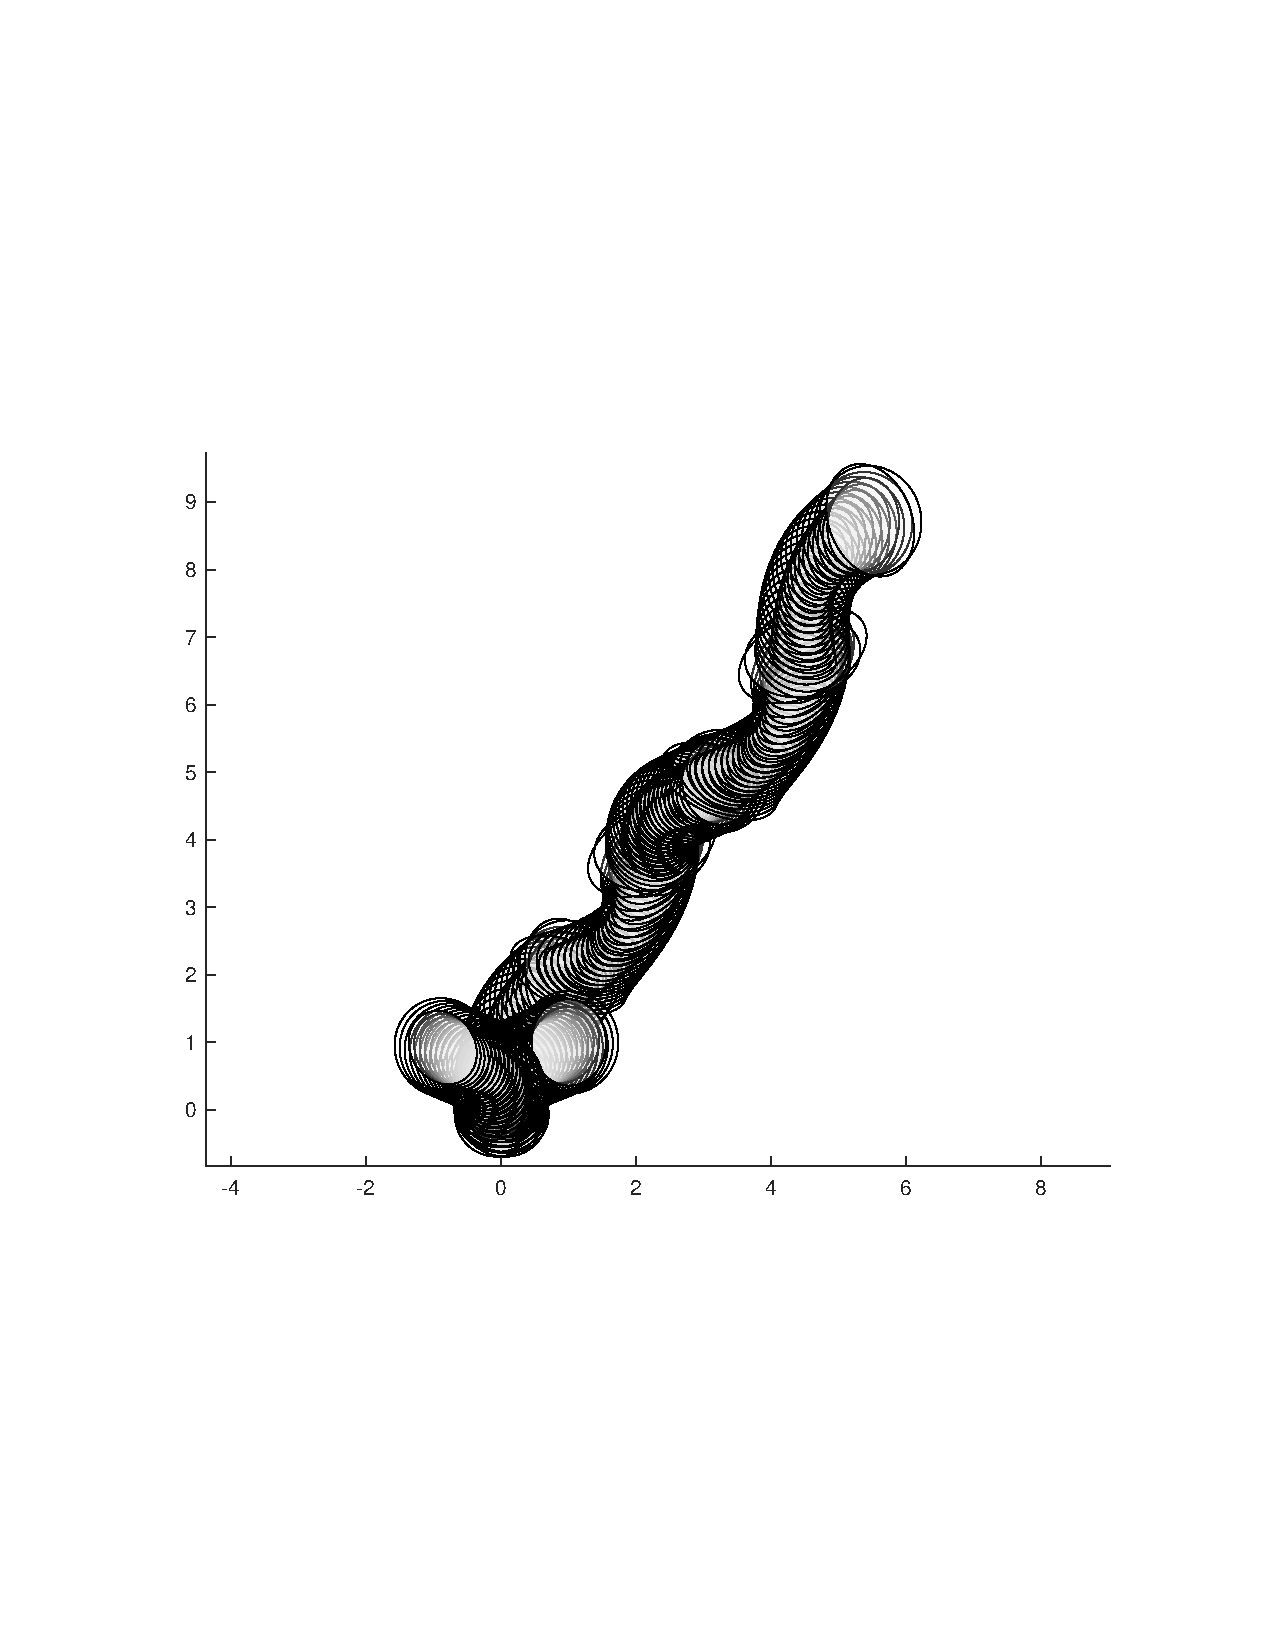
\includegraphics[scale=.4, trim={0cm 7cm 0cm
    7cm}]{figures/method/funnel-tree} \caption[A tree of funnels built by the
  \rrtfunnel{} algorithm]{A tree of funnels built by the \rrtfunnel{} algorithm,
    showing how longer motion primitives are built up from primitives in the
    basis set.}
  \label{fig:funnel-composition-tree}
\end{figure}


\subsection{Invariance of the Funnels Calculated}

The funnels generated are \textit{outer approximations} of reachable sets for
the system at hand~\cite{majumdarFunnelLibrariesRealtime2017}. This means that
in general they are larger than the actual reachable set for the system. This
can be verified through a Monte-Carlo simulation. Running N-simulations from the
funnel inlet, and storing the solutions, it is possible to visualize the actual
funnel for the system, an example of which can be seen in
\cref{fig:funnel-simulated-overlaid}.

By comparing one of the funnels in the funnel set with a funnel based from
\(10.000\) simulation runs, it is seen that the calculated funnels are indeed
proper outer approximations of the time-reachable sets for the uncertain
dynamical system. Therefore, the conclusion is that the uncertain trajectories
are contained within the funnels used in the planner, and the trajectories can
be seen as robust to uncertainty given the uncertainty and dynamical assumptions
made.

\section{RRT}
\label{sec:RRT}

With the basic framework for dealing with funnels as motion primitives
constructed, it is time to build the \ac{RRT} part of the \rrtfunnel{}
algorithm. The reason for basing the global path planning framework on the
\ac{RRT} motion planning algorithm are as follows. One, it has the ability to
quickly expand deep into the search-space, and then later progress towards a
finer sampling, which is valuable as it avoids local minima. Two, the \ac{RRT}
algorithm is easily extensible to larger state spaces, and thus adding to the
generality of the \rrtfunnel{} algorithm, such that it can be adapted to fit a
wide range of dynamical systems, while at the same time it has only three main
components that needs to be in place in order for successful path planning to
happen in an arbitrary configuration space. Namely, a suitable probability
distribution to sample from, and a distance metric for the nearest neighbor and
the extension step. The \ac{RRT} algorithm is beneficial as most of the
complexity accompanied with the planning problem (like uncertainty and
controller calculations) has already been handled by the \ac{SOS} framework, and
hence the \ac{RRT} algorithm need only concern itself with stacking one robust
motion primitive after the other without any concern for the complexities
mentioned above.

\subsection{Distance in Configuration Space}

The \rrtfunnel{} algorithm will use the same metric for both the closest node
and the extend operation on the funnel graph. The metric chosen is a modified
Euclidean metric which weights the angle \(\theta\) depending on how close the
airplane is to the final configuration, and is defined as
\[
  \rho(\vect{x}_{1}, \vect{x}_{2}) = w_{1}\norm{\mathnormal{X_{1}} -
    \mathnormal{X_{2}}} + w_{2}f(\theta_1,\theta_2) ,
\]
where \(\norm{\mathnormal{X_{1}} - \mathnormal{X_{2}}}\) is the standard
Euclidean metric, \(f\) is a function giving the distance between
headings~\cite{kuffnerEffectiveSamplingDistance2004}. The rotations and distance
is then scaled relative to the translation distance. Which helps solve some of
the problems with the Euclidean distance metric.

\subsection{The Funnel-Graph}

Even though the \rrtfunnel{} algorithm can work just fine with a collection of
funnels, and simply brute-force all funnels at the planning stage, it is helpful
to associate some kind of structure with the collection. Therefore the funnels
will be organized into a graph structure \(\mathcal{G}\) where each funnel is an
edge in the graph, and the inlets and the outlets are vertices. The planner
needs information about which funnels that are composable, as they may not all
be composable with each other, implying that the resultant graph is not
necessarily complete.

\begin{figure}[!t]
  \begin{minipage}[c]{.45\columnwidth}
    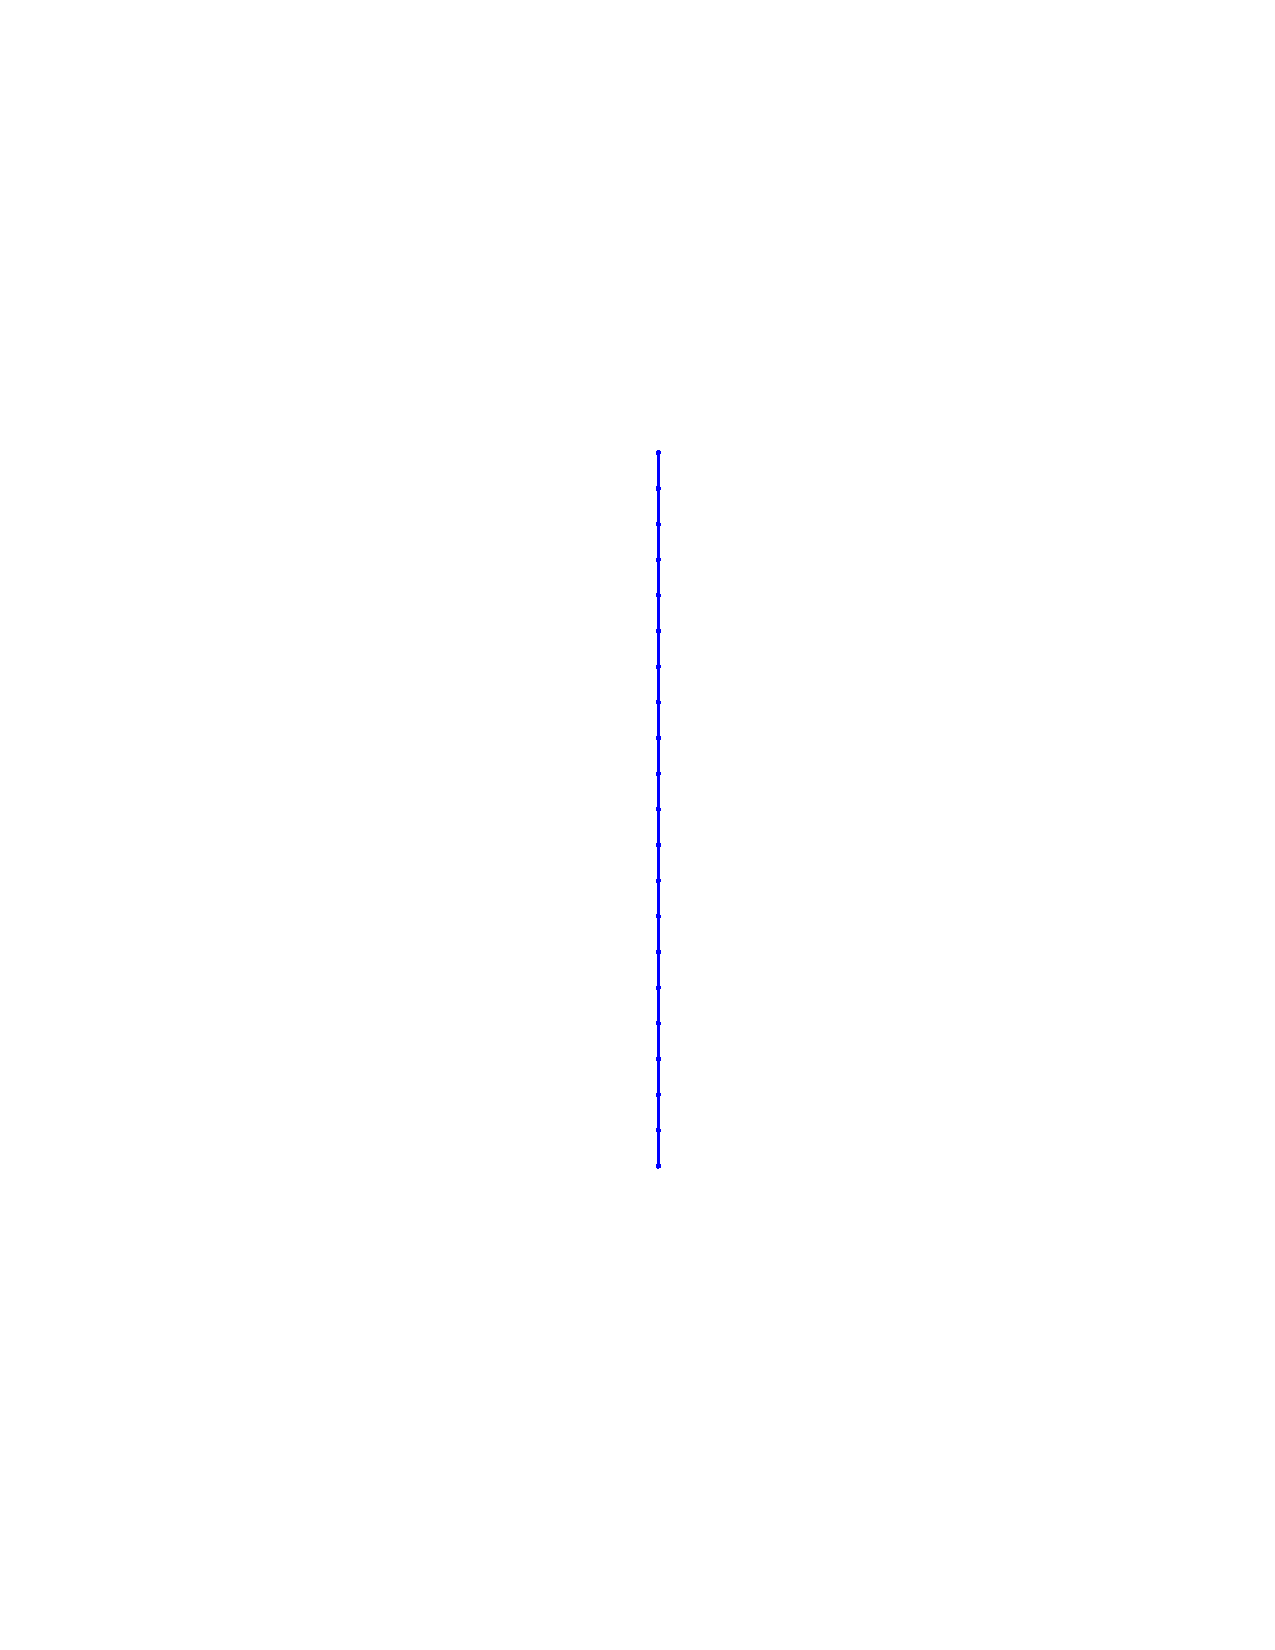
\includegraphics[trim={5cm 5cm 5cm 5cm},
    width=.9\columnwidth]{figures/method/trajectory-sampled}
    \caption{Trajectory sampled 21 times.}
  \end{minipage} \; %
  \begin{minipage}[c]{.45\columnwidth}
    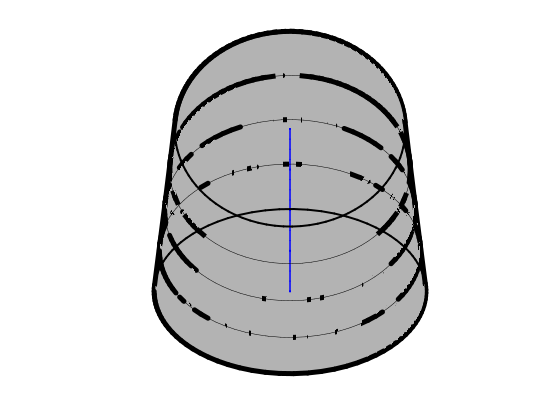
\includegraphics[trim={5cm 5cm 5cm 5cm},
    width=.9\columnwidth]{figures/method/funnel-sampled}
    \caption{The verified trajectory ellipsis overlaid at the sample times.}
    \label{fig:funnel-straight-sampled}
  \end{minipage}
\end{figure}

Composition of funnels is verified using \cref{def:invarant-funnel-composition},
and the composability graph is built using \cref{alg:create-funnel-graph} on
page~\pageref{alg:create-funnel-graph}.

\begin{figure}[!t]
  \caption{Check funnel composability}
  \label{alg:create-funnel-graph}
  \begin{algorithmic}[0]
    \Procedure{CheckFunnelComposability}{\(\mathcal{F} \rightarrow
      \mathcal{G}(\mathcal{F})\)} \Comment{Takes \(\mathcal{F}\), the basic set
      of funnels, and returns \(\mathcal{G}\), a directed graph, representing
      the composability of the funnels.}
    \For{ \(F_{i} \in \mathcal{F}\)}
    \For {\(F_{j} \in \mathcal{F}\)}
    \If {\(F_{i(t_{0})} \subset F_{j}(t_{\mathit{end}})\)}
      \State \(\mathcal{G} \leftarrow{} \left( F_{i}(t_{0}), F_{j}(t_{end})
      \right)\)
    \EndIf
    \EndFor
    \EndFor
    \EndProcedure
  \end{algorithmic}
\end{figure}

\subsection{The \rrtfunnel{} Algorithm}

With the basic framework finished, it is time to introduce the formulation of
the \rrtfunnel{} algorithm itself. The \rrtfunnel{} algorithm is a modified
\ac{RRT} algorithm which employs the precomputed funnels as motion primitives
for its expansion operator, and pseudocode for its definition can be found in
\cref{alg:rrtfunnel} on page~\pageref{alg:rrtfunnel}.

\subsection{Expanding the Size of the Funnels}

In general the funnels generated are computed for the point model in
\cref{eq:dynamicalsystem} only, and hence, in order to run the experiment with a
model of some size, the funnels have to be expanded by the largest radius of the
given model. As the funnels are ellipsis surrounding the point at the trajectory
that they verify, the funnels can be expanded by any radius with a linear
transformation (like to the unit circle, expand by the wanted radii, and then
transform back). An expansion of the point model funnel can be seen in
\cref{fig:expanded-funnel}.


\begin{figure}[!t]
  \centering 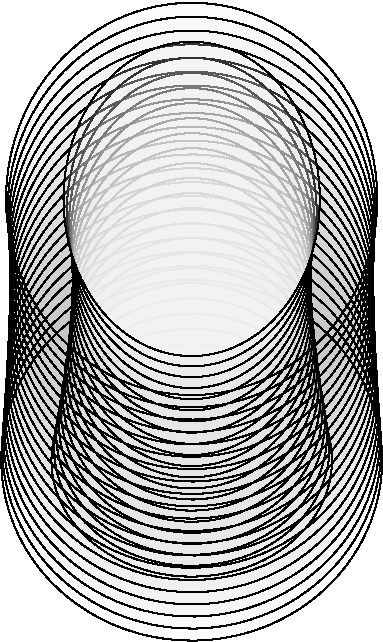
\includegraphics[scale=.5]{figures/method/expanded-funnel}
  \caption[The expanded experiment funnel]{The original funnel created from the point model, with a funnel
    expanded by a radius of 0.1 surrounding it.}
  \label{fig:expanded-funnel}
\end{figure}

\subsection{Funnel Composition}
\label{subsec:funnel-no-composable}

In accordance with \cref{sec:composable-funnels}, the funnel robustness
guarantees are only valid if the funnels are composable as per
\cref{def:invarant-funnel-composition}. Unfortunately, the funnels do not
compose as per this definition in the experiments run, and the composition
testing of the algorithm has to be left out. Thus the experiments are run with a
funnel graph that is complete, and all funnels can compose with each other, at
the cost of the mathematical robustness guarantees of the system. This is
because the one dimensional controller employed has no influence on the speed of
the airplane, and hence there is no way to make the system converge in the
direction of speed as exemplified in the~\cref{fig:funnel-conv}. This is further
exemplified in \cref{fig:funnel-inlet-outlet}, where the inlet is overlaid the
outlets for the projected xy-funnel, and it can be seen that the controller is
able to converge the xy-funnel in the x-direction, but not in the y-direction,
as it has no control over this dimension at all. The framework can be expanded
with this functionality however, but this will be referred to as future work.

\begin{figure}[!t]
  \centering
  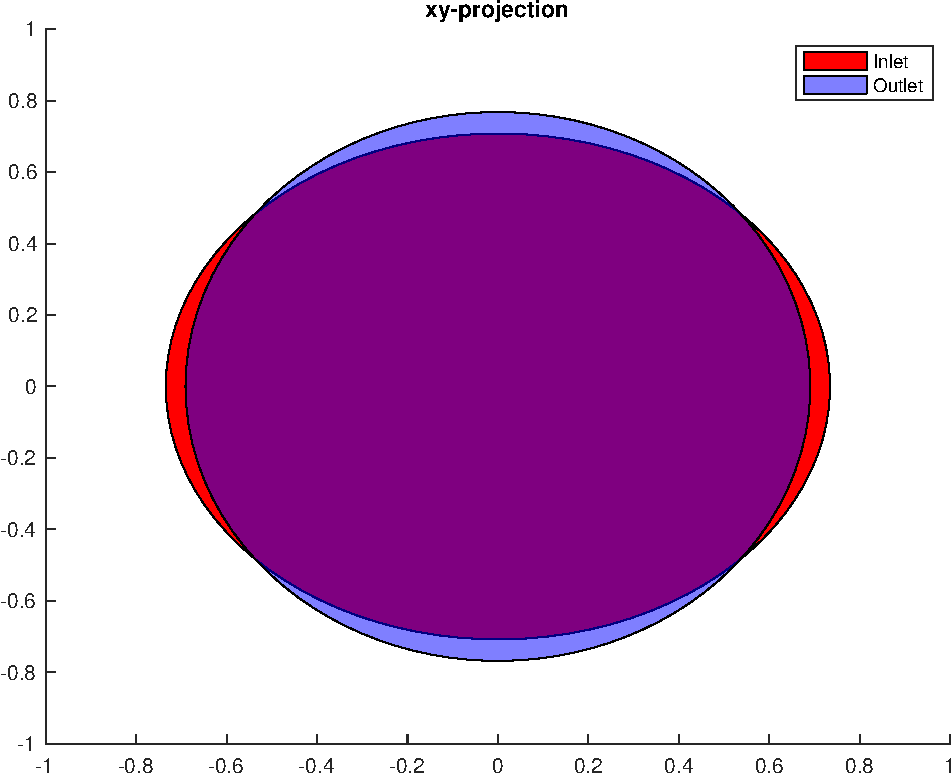
\includegraphics[width=.8\columnwidth]{figures/experiments/funnel-inlet-outlet}
  \caption[The projection of the funnel inlet and outlet in the xy-plane]{The projection of the funnel inlet and outlet in the xy-plane. It is
    seen that the controller is able to make the funnel converge in the
    x-direction as expected, however, it has no control in the y-direction, as
    there is no controller steering the speed of the vehicle.}
  \label{fig:funnel-inlet-outlet}
\end{figure}

\subsection{Continuous Verification of Invariance}
\label{subsec:check-vehicle-in-funnel}

% \begin{figure}
%   \centering
%   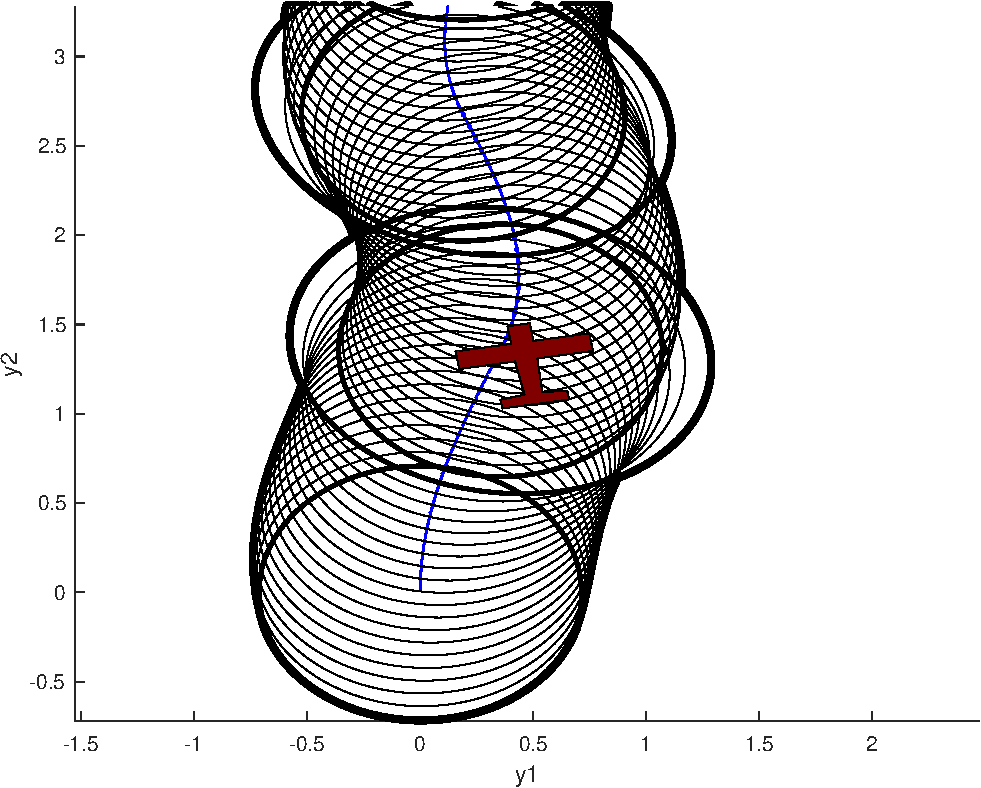
\includegraphics[width=.8\textwidth]{figures/experiments/airplane-in-funnel} \caption[A
%   figure of the airplane in the funnel]{A figure of the airplane in the funnel
%     projected down on the xy-plane during a simulation run.}
% \end{figure}
In order to remedy this off-line compositional robustness guarantees, the
\rrtfunnel{} algorithm will keep track of whether the model has left the funnel
during execution, and aborts the simulation with the emergency maneuver if the
airplane leaves one of the funnels at runtime. This happens if the value of the
Lyapunov function is larger than one. This will be counted in the experiments as
a collision on the part of the \rrtfunnel{} algorithm. A plot of the Lyapunov
values for a simulation run can be seen in \cref{fig:lyapunov-values}.

\begin{figure}[!t]
  \centering
  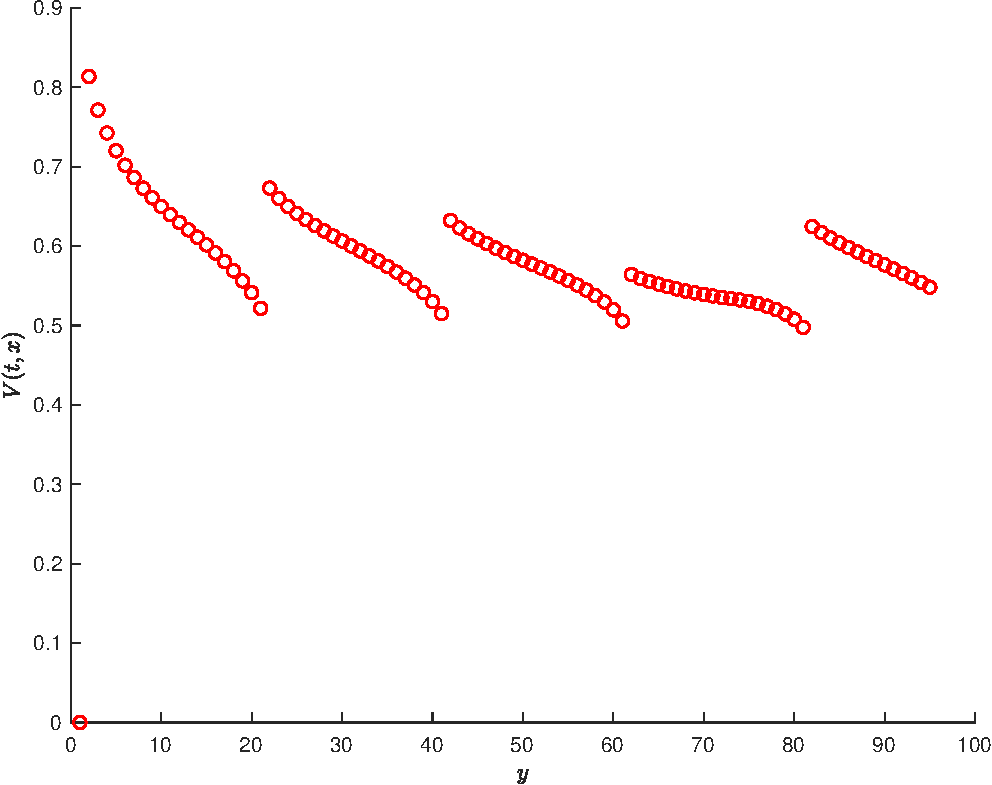
\includegraphics[width=.8\columnwidth]{figures/experiments/lyapunov-values-simulation-run}
  \caption[A plot of the Lyapunov values for an experiment]{The plot of the Lyapunov values for a simulation run at the sampling
    times \(t_k\).}
  \label{fig:lyapunov-values}
\end{figure}

\subsection{The Obstacle Forest}
\label{sec:Poisson-Process}

In order to generate the obstacle field, which is to resemble a forest, a
\textit{spatial Poisson process} is employed. Poisson processes are used to
model random configurations of points in space, and hence are well suited for
generating a different obstacle forest for each simulation
run~\cite{Kroese_2014}. For the experiments below, a forest will be the special
case of realizing a spatial Poisson process on \(\R^2\).

A Poisson process requires a few key parameters. Firstly, \(\lambda\) is the
intensity of the spatial process, deciding the density of the generated forest,
and hence the difficulty in traversing it. For these experiments, the intensity
will be held constant for each experiment run, and not vary with points in space
i.e. the process is homogeneous.

\begin{definition}{Generating a Poisson random measure}
  \label{def:Poisson-def}
  \begin{enumerate}
  \item Generate a Poisson random variable \(N \sim \poi \bigl( \mu(E) \bigr) \).
  \item Draw \(X_1,X_2,\ldots,X_N \sim g\), where \(g(\vect{x}) =
    \lambda(\vect{x})/ \mu(E)\).
  \end{enumerate}
\end{definition}
Here \(E\) is the set over which the points should be generated, and the
\textit{probability distribution function} \(g(x_1, x_2) =
\lambda(\vect{x})/\mu(E)\)~\cite[Definition~1.1.1]{Kroese_2014}. Finally,
\(\mu(E)\) is defined as
\[
  \mu(E) = \int_{E} \lambda(\vect{x})\, \mathrm{d} \vect{x} \mathEoS
\]
For the experiments the set \(E\) will be a square defined as \(E =
{[-\alpha, \alpha]}^2 \) of which the resultant forest on a \(20 \times 20\)
grid can be seen in figure~\cref{fig:poisson009}.

\subsection{The Size of the Airplane and the Obstacles Models}
\label{subsec:deciding-model-size}

The funnels generated thus far are created from a point model of the airplane,
and its dynamics. If the grid that the simulations are run on are set to have an
unit size of one meter, then the funnels from the basic set are given a velocity
of \([v(t)] = \IEEEunit{m/s}\), \([\theta] = \IEEEunit{rad}\), and \([\dot{\theta}]
= \IEEEunit{rad/s}\), where \( [\, \cdot \,] \) is the unit operator. The
size of the airplane is arbitrary, and can be chosen freely, but if it is
imagined as a radio controlled aircraft, with a speed of \(10}\) \IEEEunit{m/s},
then a size of \(10 \times 20 \) \IEEEunit{c/m} keeps everything within the
realm of a normal radio controlled aircraft and its capabilities. The mass is
not relevant for our first order dynamics, but still the airplane is assigned a
mass of \(1\, \textit{kilo}\), so that the translation of the model dynamics is not
irrelevant. A figure of the airplane can be seen in \cref{fig:radio-vehicle}.

\subsection{Expanding the Funnels around the Airplane Model}
\label{subsec:expand-funnel}

The size of the airplane in the original model is a single point, and as such,
the expanded airplane model is not accounted for in the current funnels.
Therefore the funnels have to be expanded in order for them to accommodate the
necessary robustness guarantees that are expected from the algorithm. However,
the size of the airplane only affects the size of the funnel ellipsis projected
down into the xy-plane. Therefore, first extract the projected size of the
funnel, through a projection map: \(P \colon \R^4 \rightarrow \R^2\), where \(P
= \begin{bmatrix} I_{2 \times 2} & {0}_{2 \times 2} \\ \end{bmatrix} \) such
that for the projected ellipsoid
\(
  \mathcal{E}_{p} = \set{\bar{\vect{x}} \in \R^{2} \mid
    {\bar{\vect{x}}}^{T}S_{k}^{(p)}\bar{\vect{x}} \leq 1},
\)
with \(S_{k}^{(p)}\) given by
\(
  S_{k}^{(p)} = {\left( PS_{k}^{-1}P^T \right)}^{-1},
\)
is the set containing the funnel projected down into the xy-plane. Here
\(\mathcal{E}_{p}\) is the projected set of the ellipsoid in the xy-plane
as is seen in \cref{subsec:xy-cost-function}. In general an ellipse centered at
the origin is a linear transformation of the unit circle~\cite{lay2005linear}.
Exploiting this fact, the funnel ellipsoids can be expanded to encompass the
airplane model. Take note that the matrix \(S_{k}\) is
\textit{Positive semidefinite}, and hence can be Cholezky
factorized~\cite{lay2005linear}. Then expanded ellipsis (which now contains all
the possible states of the airplane model) is given by:
\begin{align*}
  S_{k}^{(\mathcal{P})} &= R^{T}R \\
  \vect{x} &= R^{-1}\vect{y} \\
  \mathcal{C} &= \set{\vect{y} \in \R^2 \mid \vect{y}^{T}\vect{y} \leq 1 + r_{a}} \\
  \mathcal{E}_{\mathit{exp}} &= \set{R^{-1}\vect{y} \mid \vect{y} \in \mathcal{C}} \\
\end{align*}
where \(\mathcal{E}_{\mathit{exp}}\) are the ellipsoids which contains the
volume of the airplane for all verified states in the funnel, and
\(r_{\mathit{a}}\) is the widest part of the model at hand, which in this case
is the wingspan. A picture of the initial funnel and the funnel expanded around
the airplane model can be seen in
figure~\cref{fig:expanded-funnel,fig:expanded-and-unexpanded}.

\subsection{The Initial Motion Primitive Set}
\label{subsec:initial-motion-primitive}

The basis set of motion primitives should be small, yet cover enough of the
finer movements of the airplane so that the motion of the airplane can be near
continuous when composed together. Thus in order to generate a dense set of
motion primitives \cref{alg:initial-motion-primitives-generation} is employed in
order to generate points along the arc of a circle with \(N\) different radii as
the initial points for the trajectory generator described in
\cref{subsec:generating-the-trajectories}. The initial trajectories employed in
the experiments can be seen in \cref{fig:intial-trajectories-exp}.

\begin{figure}[!t]
  \caption{Generating the initial motion primitives}
  \label{alg:initial-motion-primitives-generation}
  \DontPrintSemicolon \SetAlgoNoLine

  \KwIn{%
    \(n\) - Number of points along the arch \\
    \(r_{0}\) - Initial radius \\
    \(r_{f}\) - Final radius \\
    \(s\) - Step-size (\(r_{n+1} = r_{n} + s\)) } \KwOut{\(\mathbf{X}\) -
    Endpoints matrix for the trajectory generator}

  \(\theta_{0} = \pi\) \;

  \For{\(r_{k+1} = r_{k} + s\)}{ \(\theta_{j} = \frac{\theta_{0}}{2r}\) \;
    \(\theta_{stepsize} = \frac{\theta{j}}{(n-1)/2}\) \; \(\mathbf{X} =
    (r_{k+1}, \theta=0)\) \; \For{\(i = 1 \) \KwTo \(\frac{n-1}{2}\)}{
      \(\theta_{ki} = i*\theta_{stepsize}\) \; \(\mathbf{X} = (r, \pm
      \theta_{ki})\) \; }\; }\;
\end{figure}

\begin{figure}[!t]
  \centering
  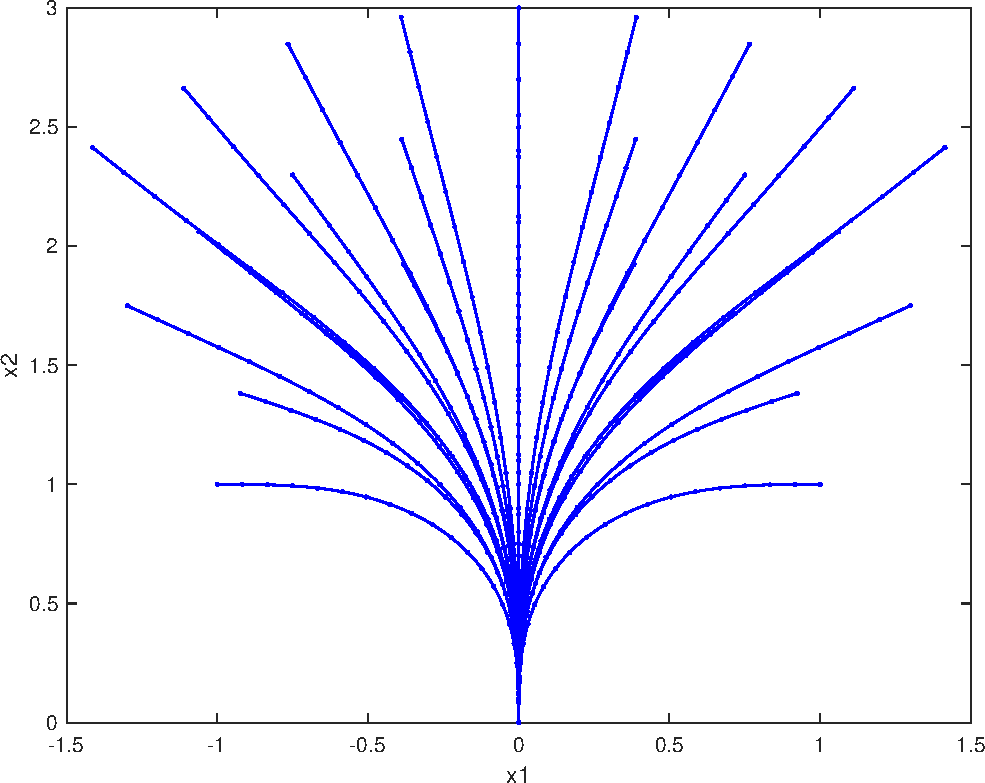
\includegraphics[width=.8\columnwidth]{figures/experiments/initial-trajectories}
  \caption[The experiment trajectory set]{The initial trajectories used in the
    \rrtfunnel{} algorithm. The endpoints are generated by
    \cref{alg:initial-motion-primitives-generation}.}
  \label{fig:intial-trajectories-exp}
\end{figure}


\section{Experiments}
\label{sec:experiments-final}

The experiments will run the \rrtfunnel{} against a benchmark regular RRT
planner with the motion primitive set pictured in
\cref{fig:intial-trajectories-exp} on the forest traversal problem pictured in
\cref{fig:simulated-forest}. The benchmark-planner is an \ac{RRT} algorithm
using the same motion primitive set as the \rrtfunnel{} algorithm, with the same
\ac{LQR} controller, and the same distance metric. The difference is that it
does not take uncertainty into account, and instead maximizes the distance to
the nearest obstacle as the extension operator \ie{}
\begin{equation}
  \max_{i}\min_{t,j} \bigl( \vect{x}_{i}(t), o_{j} \bigr)
\end{equation}
where \(x_{i}(t) \in \mathcal{T}\), is a trajectory from the basic motion
primitive set, and \(o_{j} \in \modelobstacle{}\) is an obstacle in the
configuration space \(\modelconfigurationspace{}\). Note also that in order to
guide the expansion towards the goal, a goal bias of \(0.1\) is given to the
benchmark planner.

The end goal is set so that it will not take pose into account, and will only be
concerned with getting within an \(\epsilon\) of the \((x,y)\) in the test map.
For all the experiments below, an \(\epsilon\) of 5\IEEEunit{m} is given to the
planners.

Each test-run will be run in a forest generated with the \textit{Poisson
  process} method from \cref{sec:Poisson-Process}, and an intensity parameter
\(\lambda = 0.2\).

The experiments will record the number of collisions for each algorithm across
all test-runs. The planners will run in the same environment for each test, with
the same initial starting point, but the environments will be different for each
run, as the Poisson process generating the obstacle forest is random in nature.
With this test setup the difference between a planner which takes into account
uncertainty should become evident.

Before the experiments are run, all individual funnels in the base set are run
with a hundred simulations runs from random starting positions in its inlet, to
check if the invariant holds, and that the airplane stays within the funnel at
all times. Uncertainty is added in terms of an additive noise with \(w =
0.3\) \IEEEunit{m/s} in the world x-direction.

\subsection{Experiment Setup}

The algorithm will be tested by generating a random strip of forest of depth
\(25\)\IEEEunit{m}, and then letting it, along with the benchmark algorithm find a way
through the environment to the other side, whilst being the subject of a
simulated crosswind  of \(0,3\) and \(6\) \IEEEunit{m/s}. The trees are circles
with a radius of \(0.2\) \IEEEunit{m}, and are placed randomly on the set \(O=\{
    \vect{x} \mid -50 \le x_{1} \le 50 \text{ and } 5 \le x_{2} \le 25
  \}\), as the realization of a \textit{Poisson} process with density
\(\lambda = 0.2\) on this set. For each trial run, a new forest is generated in
this random fashion, and the algorithms are given the task to traverse the
generated map, see~\cite{Kroese_2014} for an introduction to Poisson processes.

The funnels for the \rrtfunnel{} algorithm are in this case made to handle
uncertainties up to and including \(3\) \IEEEunit{m/s} in the x-direction of the airplane,
but does not currently have any control over the y-direcction (the speed). A
figure of the test environment can be seen in \cref{fig:simulated-forest}. The
\rrtfunnel{} algorithm is run with a goal bias of \(5\%\), in order to guide the
exploration of the state-space towards the other end of the planning map. Also,
a maximum of \(5000\) nodes is set as an upper treshold on both of the
algorithm's exploration trees.

The model in the experiments are imagined as being a plane, with the dimensions
shown in \cref{fig:radio-vehicle}, and the basis of trajectories employed can be
seen in \cref{fig:intial-trajectories-exp}.

\begin{figure}[!t]
  \centering
  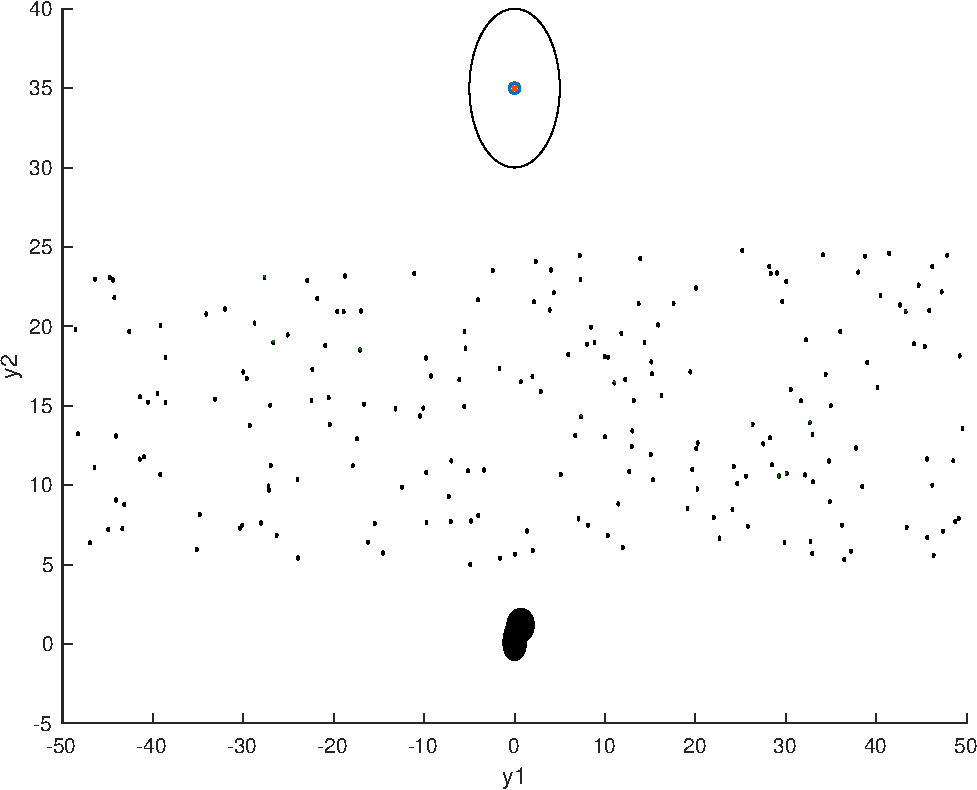
\includegraphics[width=.8\columnwidth]{figures/experiments/simulated-forest}
  \caption{The experiment environment.}
  \label{fig:simulated-forest}
\end{figure}

\subsection{Quality of the Funnels Calculated (Approximated)}

The funnels generated are \textit{outer approximations} of reachable sets for
the system at hand~\cite{majumdarFunnelLibrariesRealtime2017}. This means that
in general they are larger than the actual reachable set for the system. This
can be verified through a Monte-Carlo simulation. Running N-simulations from the
funnel inlet, and storing the solutions, it is possible to visualize the actual
funnel for the system, an example of which can be seen in
\cref{fig:funnel-simulated-overlaid}.

By comparing one of the funnels in the funnel set with a funnel based from
\(10.000\) simulation runs, it is seen that the calculated funnels are indeed
proper outer approximations of the time-reachable sets for the uncertain
dynamical system. Therefore, the conclusion is that the uncertain trajectories
are contained within the funnels used in the planner, and the trajectories can
be seen as robust to uncertainty given the uncertainty and dynamical assumptions
made.

\begin{figure}[!t]
  \begin{minipage}[r]{0.3\columnwidth}
    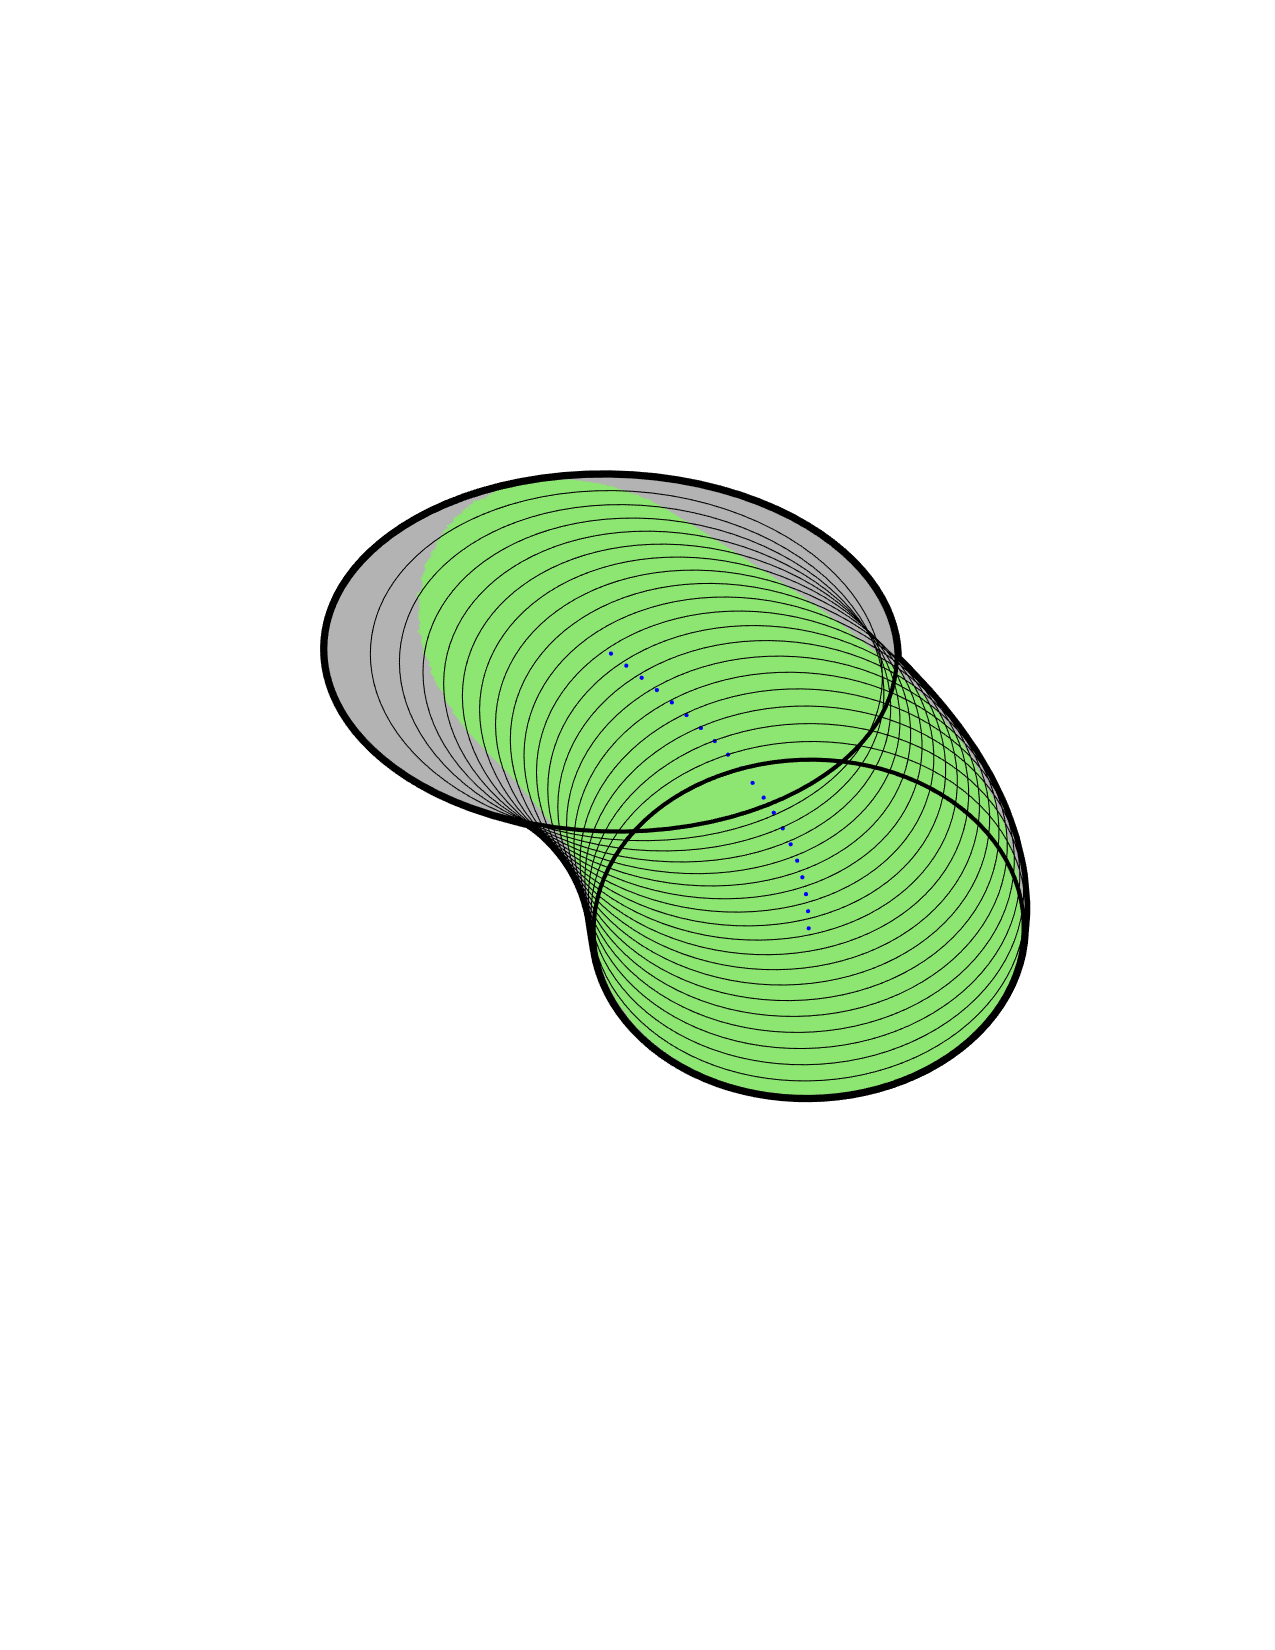
\includegraphics[width=1\columnwidth, trim={0cm 6cm 0cm
      6cm}]{figures/method/FunnelSimnew4}
  \end{minipage}
  \begin{minipage}[c]{0.3\columnwidth}
    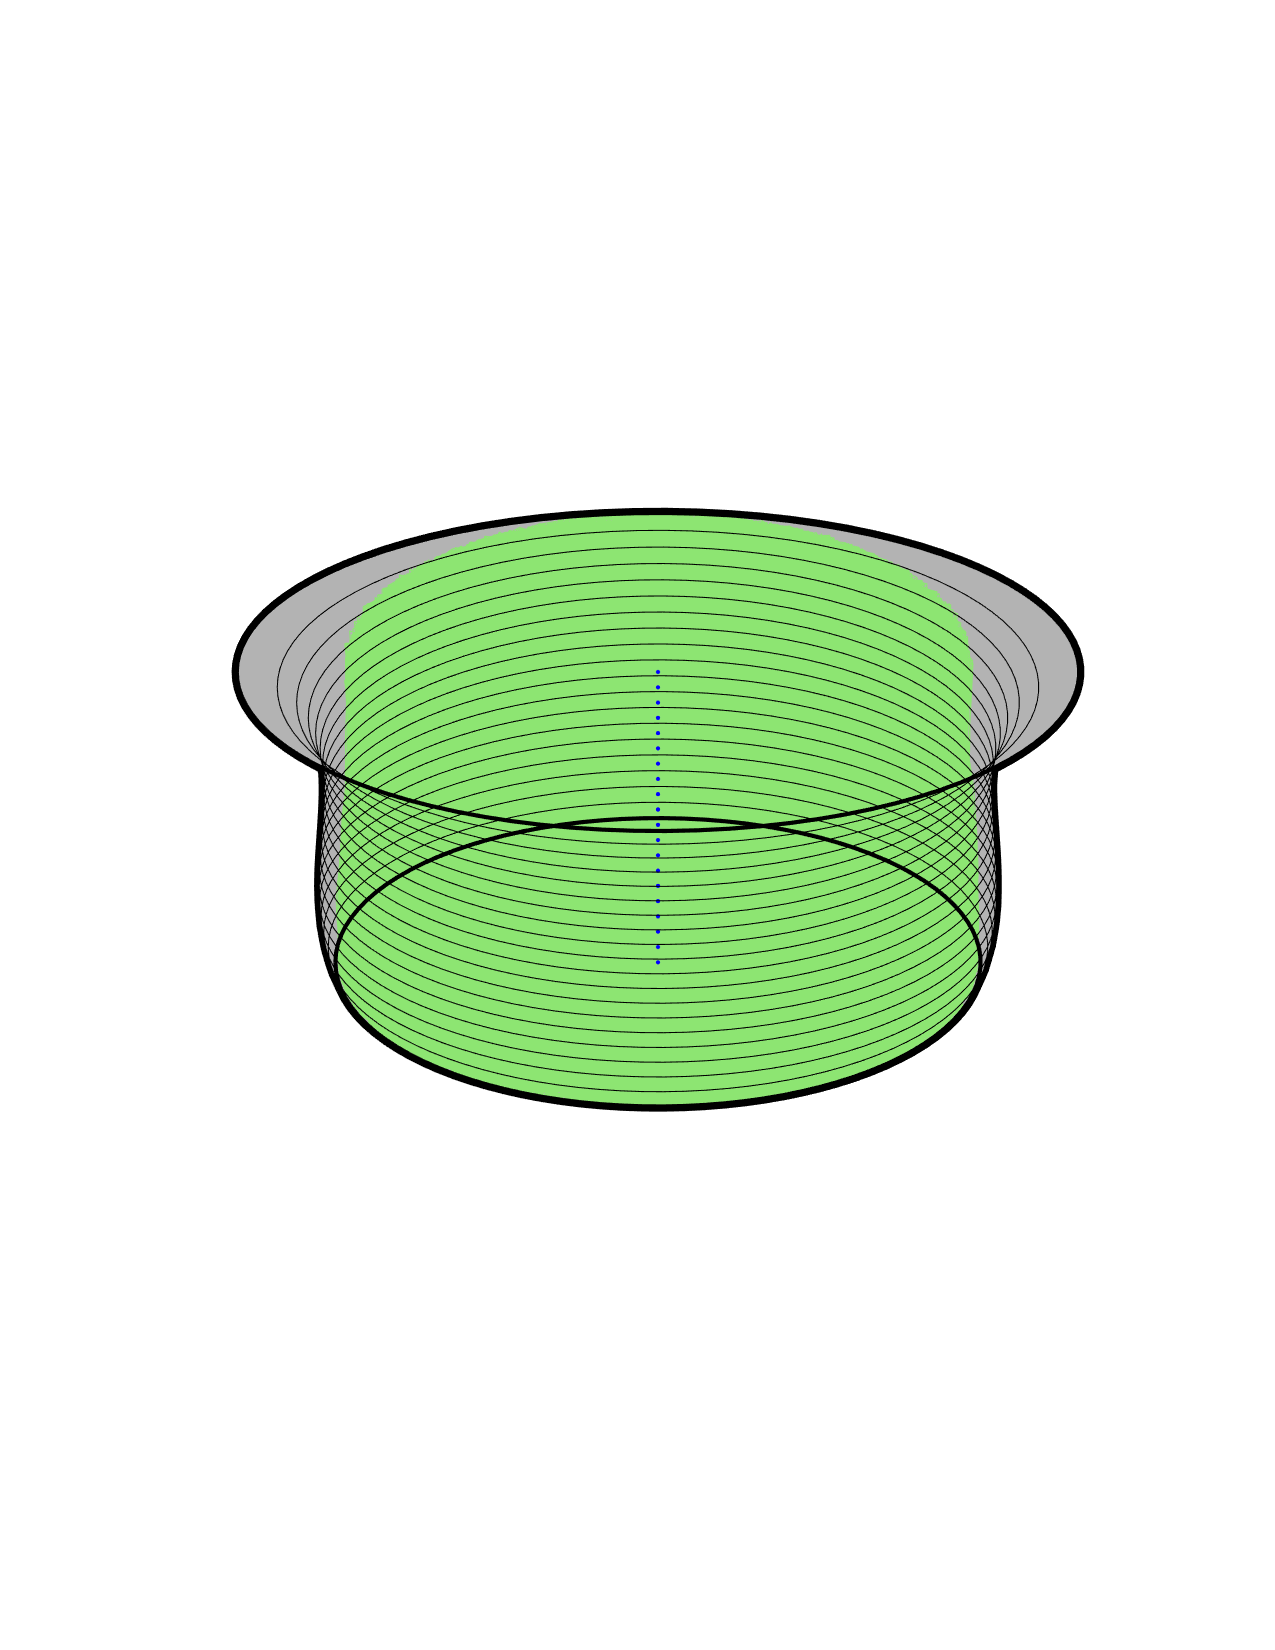
\includegraphics[width=1\columnwidth, trim={0cm 6cm 0cm
      6cm}]{figures/method/FunnelSimnew1}
  \end{minipage}
  \begin{minipage}[l]{0.3\columnwidth}
    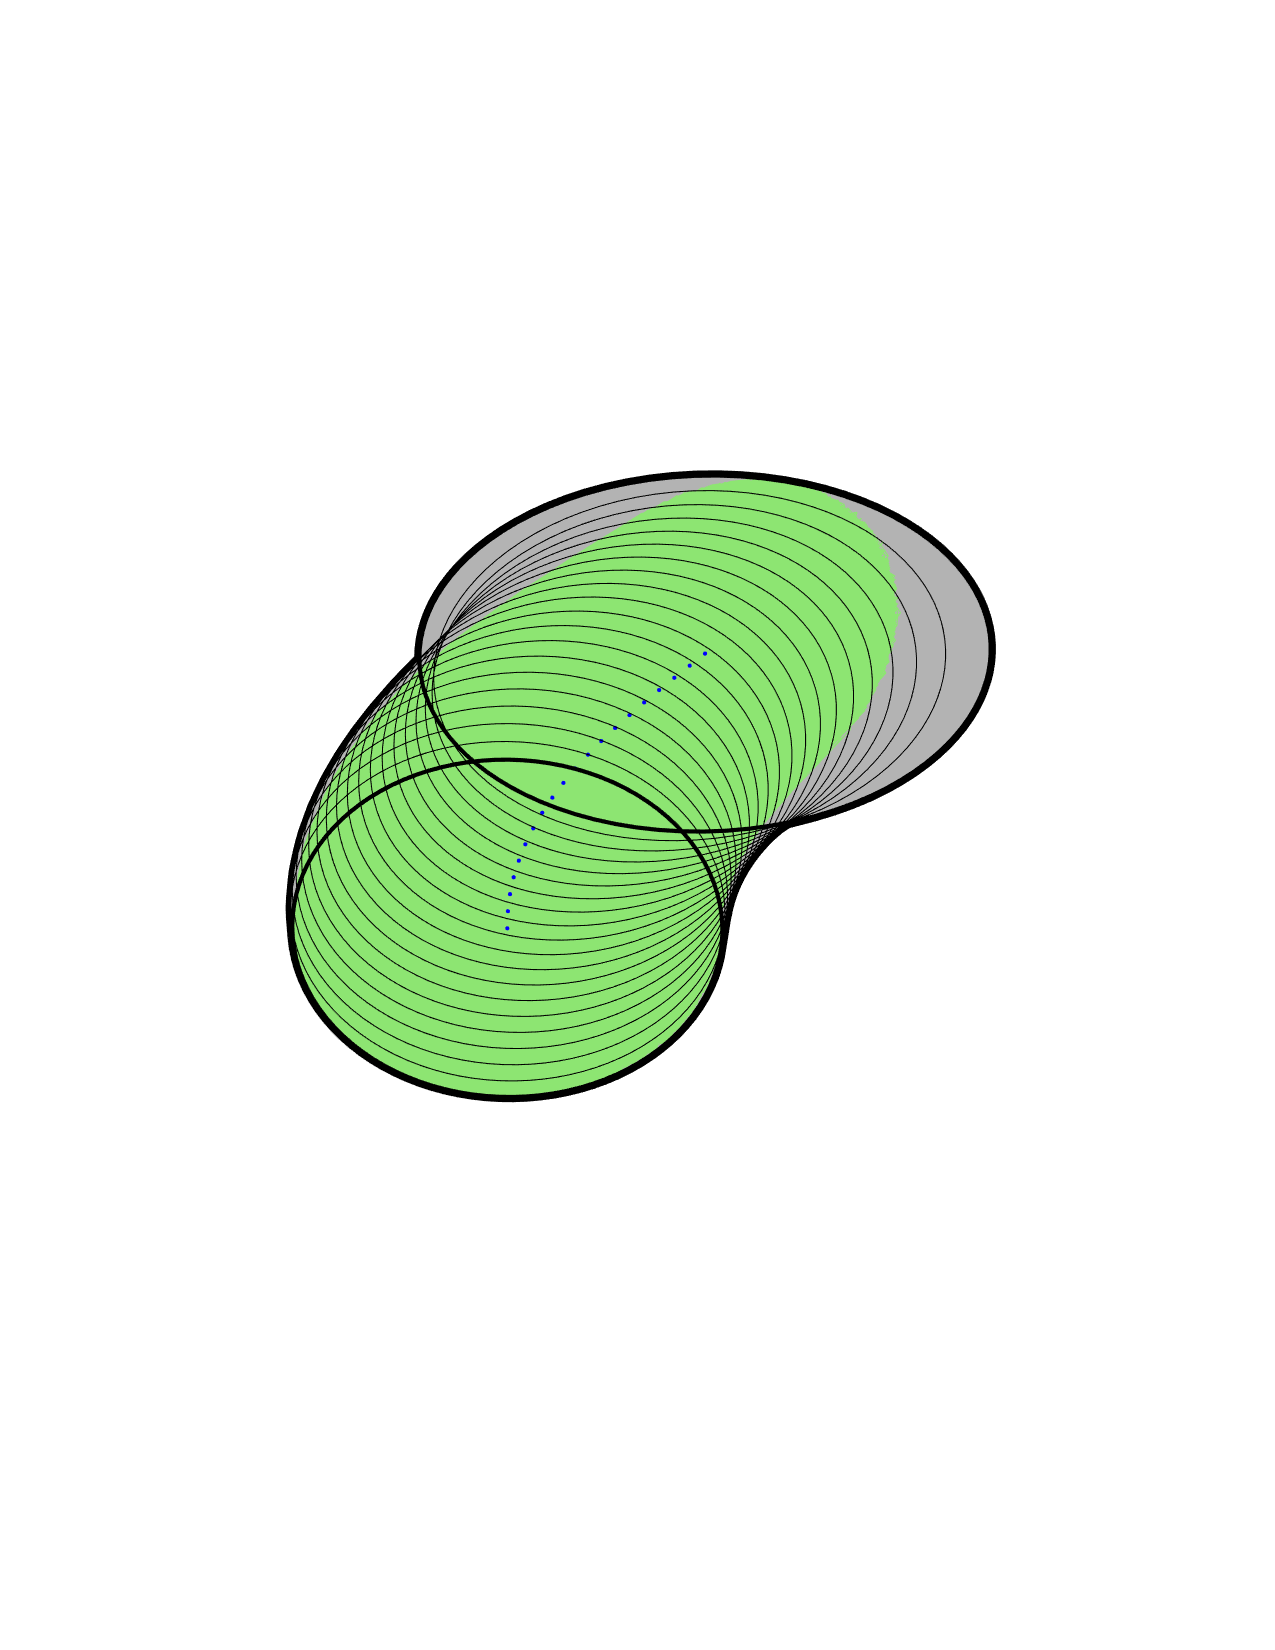
\includegraphics[width=1\columnwidth, trim={0cm 6cm 0cm
      6cm}]{figures/method/FunnelSimnew5}
  \end{minipage}
  \caption[A visualization of the simulated and the calculated reachable set]{The simulated non-polynomial system trajectories (green), overlaid
    with the outer approximation that is the funnel returned by the \ac{SOS}
    calculation (grey) for three trajectories from the trajectory library
    \(\mathcal{T}\).}
  \label{fig:funnel-simulated-overlaid}
\end{figure}

%% The expansion of the \rrtfunnel algorithm in an experiment setup can be seen in \cref{fig:rrtfunnel-expansion}. While the benchmark algorithm expansion can be seen in \cref{fig:benchmark-expansion}.

\begin{figure}[!t]
  \centering
  \begin{minipage}[c]{.9\columnwidth}
  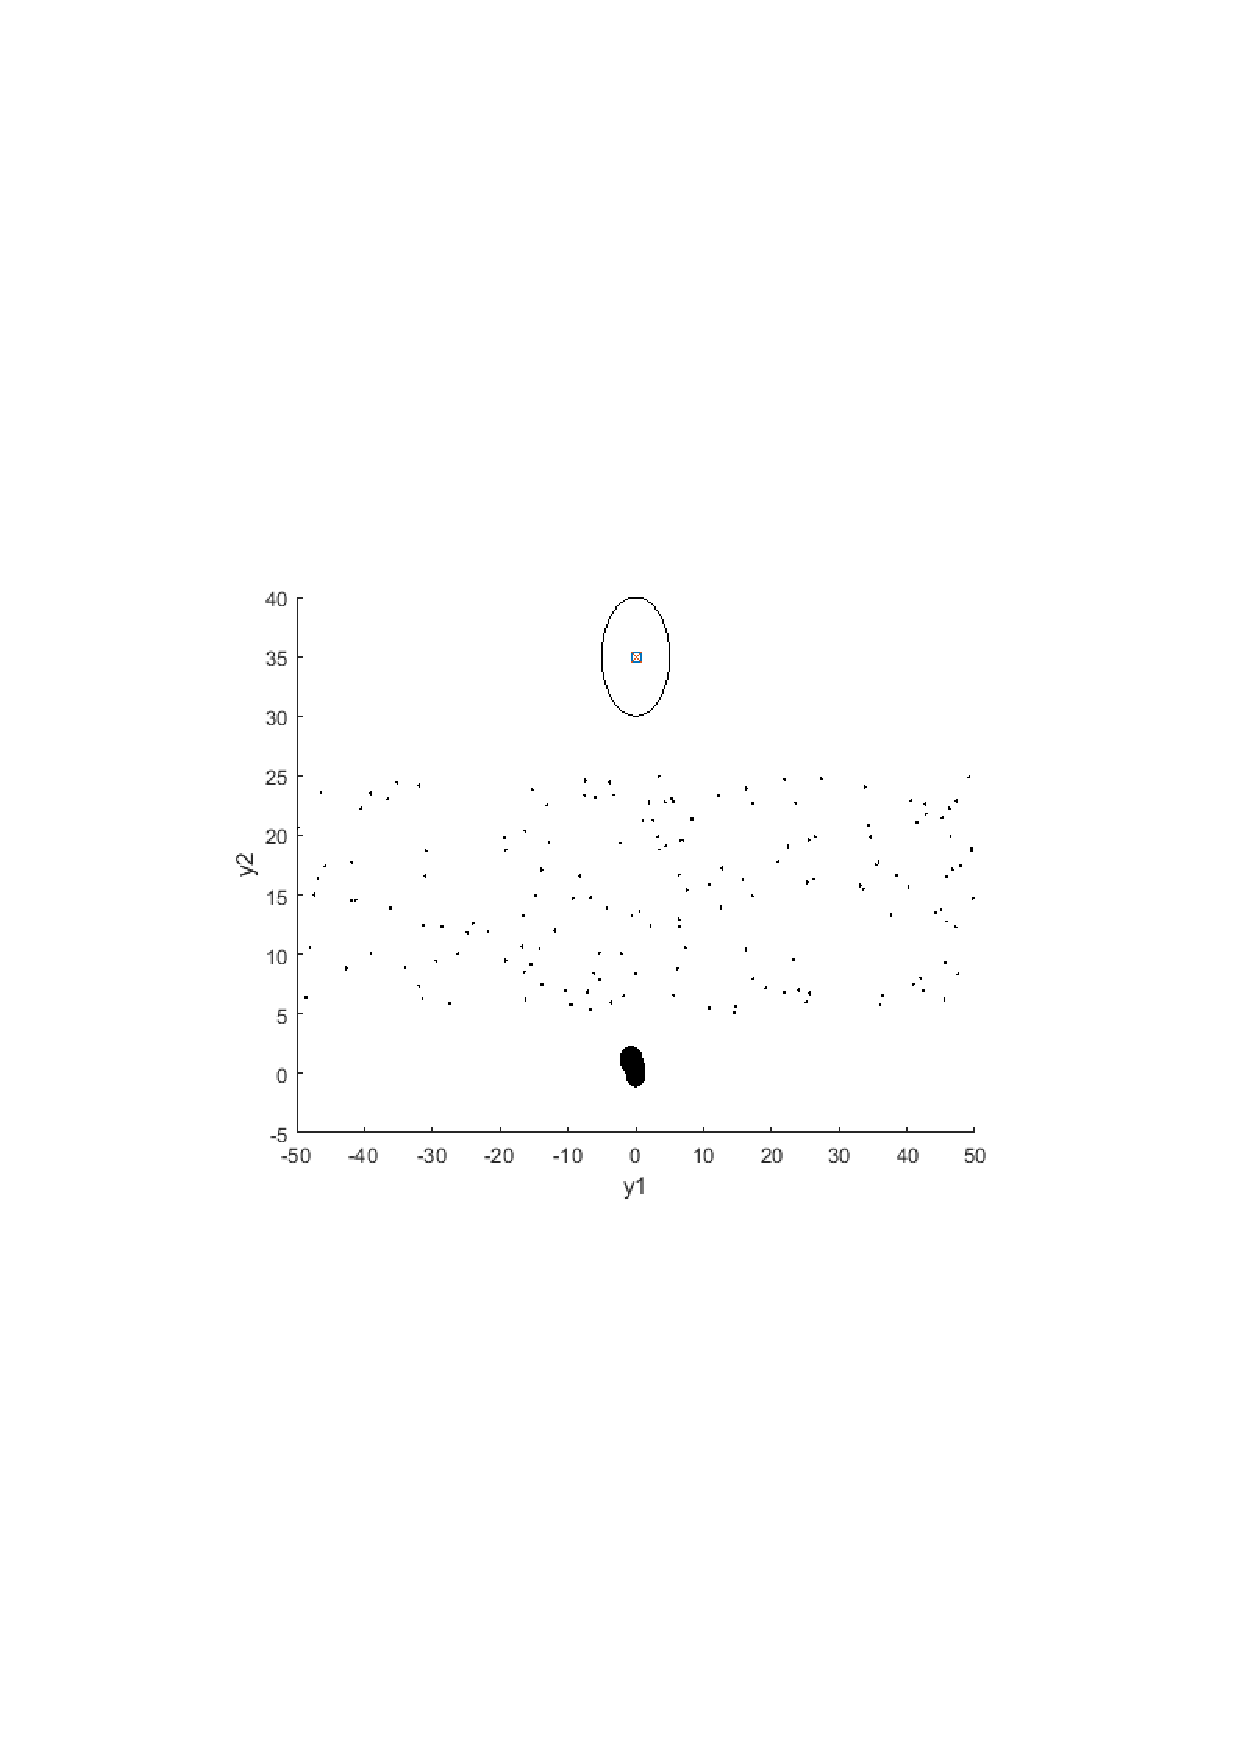
\includegraphics[scale=.5, trim={8cm, 9cm, 10cm, 7cm}]{figures/experiments/rrtfunnel-1samples.pdf}
  \caption[The expansion of the \rrtfunnel algorithm at 1, and 101 iterations]{Visualized is the expansion of the \rrtfunnel algorithm at 1 iterations of the algorithm.}
  \end{minipage}
  \newline
  \begin{minipage}[c]{.9\columnwidth}
  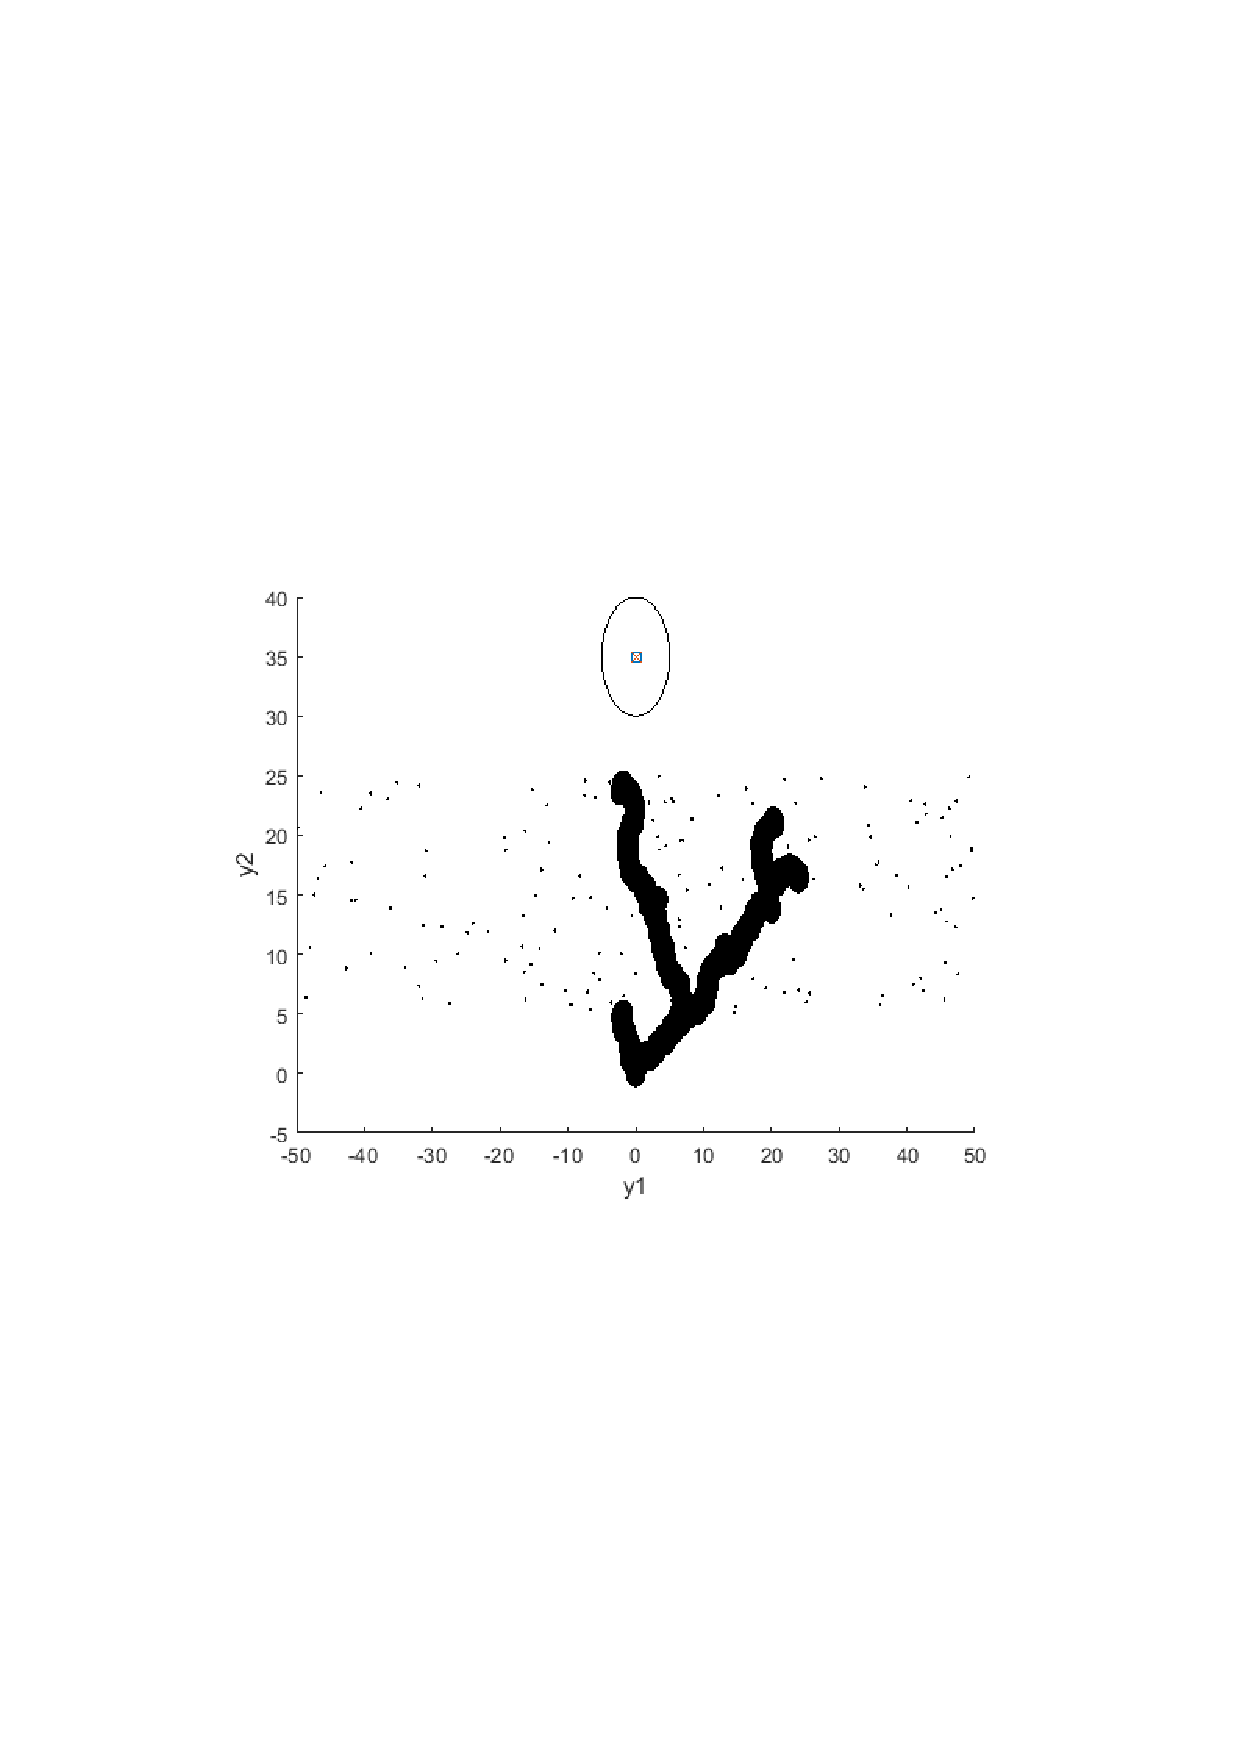
\includegraphics[scale=.5, trim={8cm, 9cm, 10cm, 7cm}]{figures/experiments/rrtfunnel-101samples.pdf}
  \caption[The expansion of the \rrtfunnel algorithm at 1, and 101 iterations]{Visualized is the expansion of the \rrtfunnel algorithm at 101 iterations of the algorithm.}
  \end{minipage}
\end{figure}

\begin{figure}[!t]
  \centering
  \begin{minipage}[c]{.8\columnwidth}
  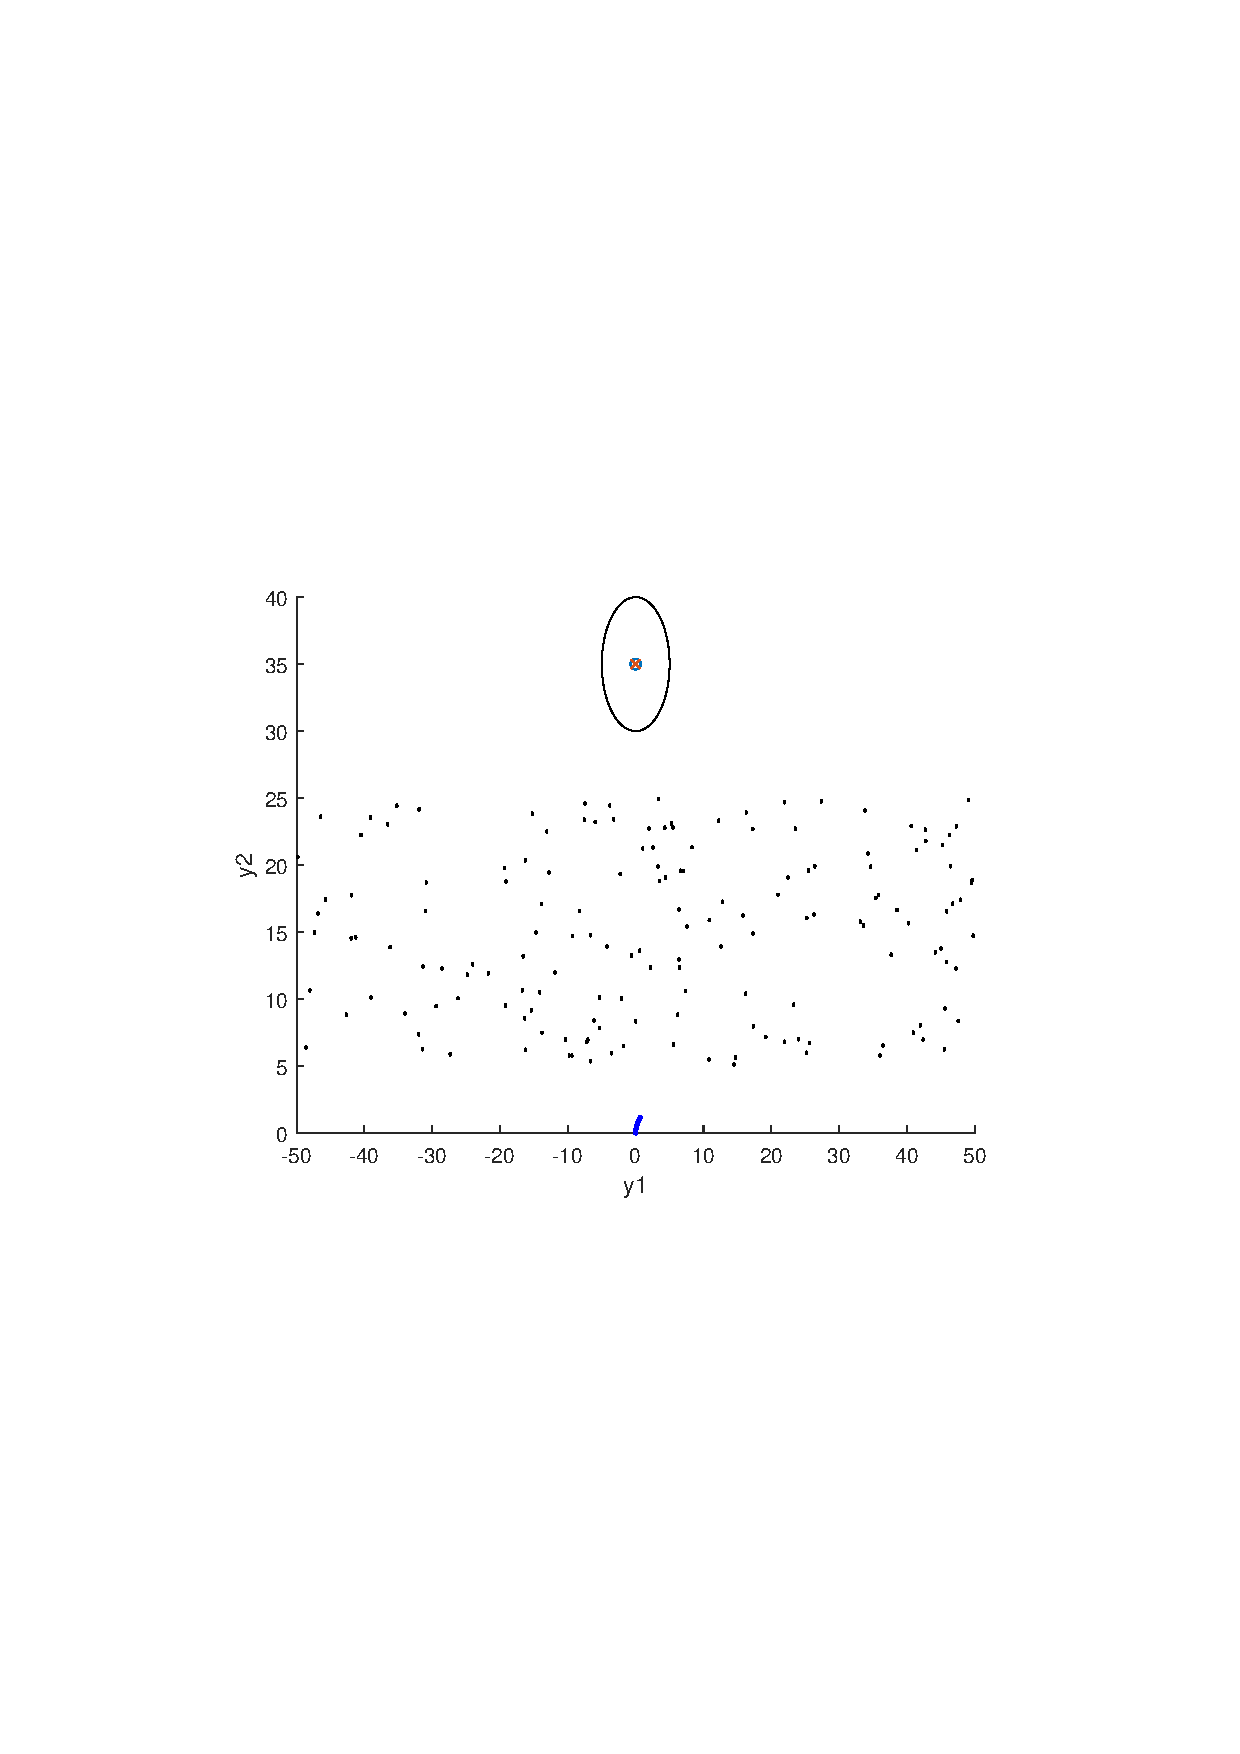
\includegraphics[width=.4\columnwidth, trim={7cm, 7cm, 7cm, 7cm}]{figures/experiments/rrtfunnel-1samples-dyn.pdf}
  \caption[The expansion of the \rrtfunnel algorithm at 1, and 101 iterations]{Visualized is the expansion of the \rrtfunnel algorithm at 1 iterations of the algorithm.}
  \end{minipage}
  \newline
  \begin{minipage}[c]{.8\columnwidth}
  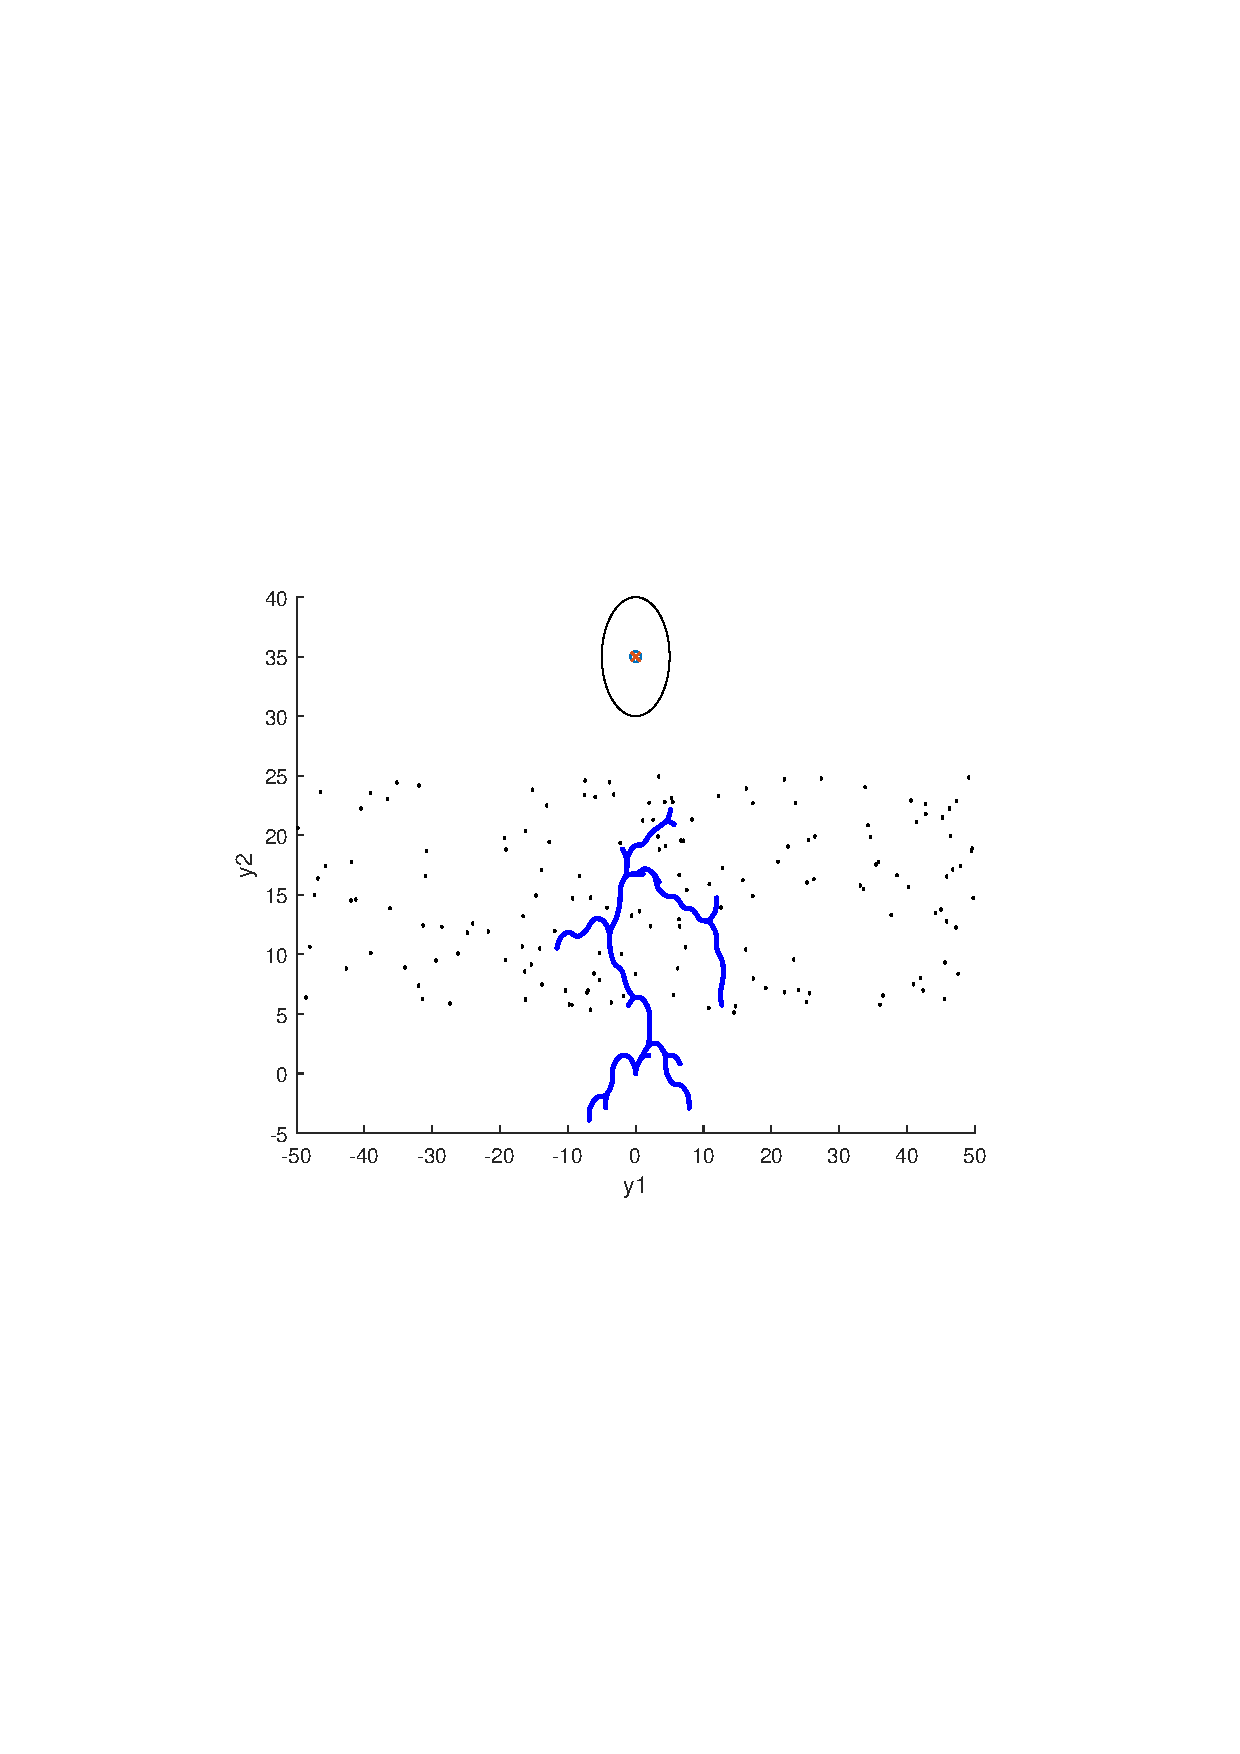
\includegraphics[width=.4\columnwidth, trim={7cm, 7cm, 7cm, 7cm}]{figures/experiments/rrtfunnel-101samples-dyn.pdf}
  \caption[The expansion of the \rrtfunnel algorithm at 1, and 101 iterations]{Visualized is the expansion of the \rrtfunnel algorithm at 101 iterations of the algorithm}
  \end{minipage}
  \newline
  \begin{minipage}[c]{.8\columnwidth}
  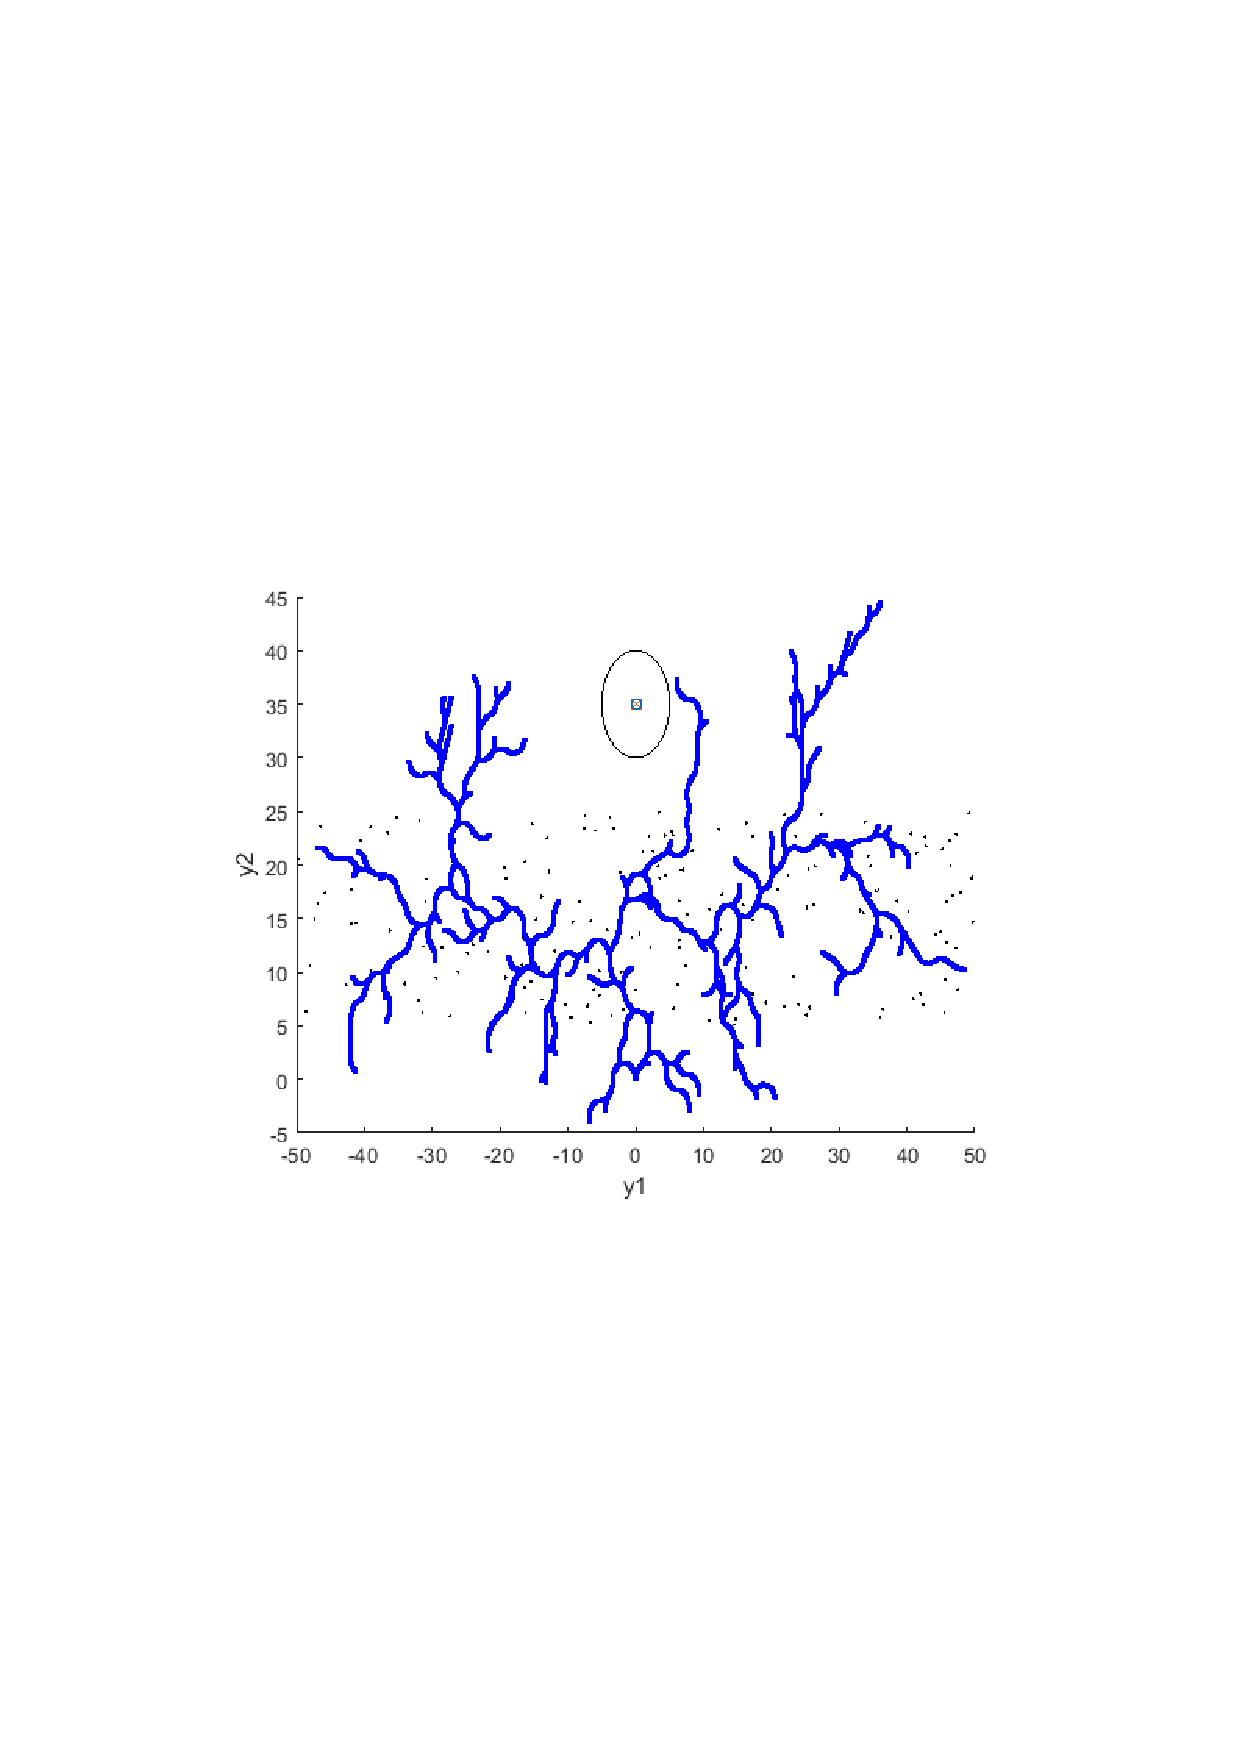
\includegraphics[width=.4\columnwidth, trim={7cm, 7cm, 7cm, 7cm}]{figures/experiments/rrtfunnel-701samples-dyn.pdf}
  \caption[The expansion of the \rrtfunnel algorithm at 1, and 101 iterations]{Visualized is the expansion of the \rrtfunnel algorithm at 701 iterations of the algorithm}
  \end{minipage}
\end{figure}
